\subsection{基域变换}

设 N 是 K 的伽罗瓦扩张， \(\Gamma\) 为 N 在 K 上的伽罗瓦群；进一步设 \(N'\) 是 \(K'\) 的伽罗瓦扩张，其伽罗瓦群为 \(\Gamma'\) 。我们将把 K（相应地， \(K'\) ）与其在 N（相应地， \(N'\) ）中的像等同。设 u 为 K 到 \(K'\) 中的同态，v 为 N 到 \(N'\) 中的同态，且 v 在 K 上的限制等于 u（参见

图 1）。设 \(\sigma \in \Gamma'\) ；由于 \(u(\mathbf{K}) \subset \mathbf{K}'\) ， \(\sigma\) 是一个 \(u(\mathbf{K})\) -自同构，作用在 \(\mathbf{N}'\) 上；此外 \(v(\mathbf{N})\) 是 \(u(\mathbf{K})\) 的伽罗瓦扩张，因此 \(\sigma\) 诱导一个 \(u(\mathbf{K})\) -自同构，作用在 \(v(\mathbf{N})\) 上（V，第55页，注记1）。换言之，对每个 \(\sigma \in \Gamma'\) ，存在唯一的元素 \(v^*(\sigma)\) 属于 \(\Gamma\) ，使得

\[
\boldsymbol {v} \circ \boldsymbol {v} ^ {*} (\sigma) = \sigma \circ \boldsymbol {v}.\tag{8}
\]

\pandocbounded{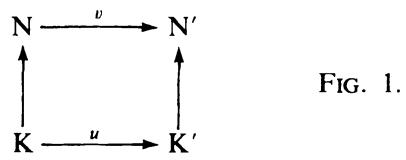
\includegraphics[keepaspectratio]{images/part002_8bfcf433.jpg}}

映射 \(v^*\) 是 \(\operatorname{Gal}(\mathbf{N}' / \mathbf{K}')\) 到 \(\operatorname{Gal}(\mathbf{N} / \mathbf{K})\) 中的同态。对每个 \(x \in \mathbf{N}\) ，映射 \(\sigma \mapsto v^*(\sigma)(x) = v^{-1}(\sigma(v(x)))\) 作为从 \(\Gamma'\) 到离散空间 \(\mathbf{N}\) 的映射是连续的，因此 \(v^*\) 是连续的。

三个特殊情形具有重要意义：

\begin{enumerate}
\def\labelenumi{\alph{enumi})}
\tightlist
\item
  若 F 是 K 的伽罗瓦扩张且 E 是 F 的一个子扩张，我们知道（V，第67页，引理1）F 是 E 的伽罗瓦扩张。让我们将前述内容应用于 N = F， \(K' = E\) ， \(N' = F\) 且 \(v = Id_{F}\) 的情形，则 \(v^{*}\) 仅仅是典范嵌入
\end{enumerate}

\[
j: \operatorname{Gal} (\mathrm{F} / \mathrm{E}) \rightarrow \operatorname{Gal} (\mathrm{F} / \mathrm{K}).
\]

这有时被称为膨胀同态。

\begin{enumerate}
\def\labelenumi{\alph{enumi})}
\setcounter{enumi}{1}
\tightlist
\item
  假设此外 E 在 K 上是伽罗瓦的。让我们将前述内容应用于 N = E， \(K' = K\) ， \(N' = F\) 且 v 是 E 到 F 中的典范嵌入的情形。则 \(v^{*}\) 正是限制同态
\end{enumerate}

\[
\pi : \operatorname{Gal} (\mathrm{F} / \mathrm{K}) \rightarrow \operatorname{Gal} (\mathrm{E} / \mathrm{K}).
\]

我们知道（V，第60页，命题3）， \(\pi\) 是满射，其核为 \(\operatorname{Gal}(\mathrm{F} / \mathrm{E})\) ，并且通过取商，它定义了从 \(\operatorname{Gal}(\mathrm{F} / \mathrm{K}) / \operatorname{Gal}(\mathrm{F} / \mathrm{E})\) 到 \(\operatorname{Gal}(\mathrm{E} / \mathrm{K})\) 上的拓扑群同构（V，第68页，推论4）。

\begin{enumerate}
\def\labelenumi{\alph{enumi})}
\setcounter{enumi}{2}
\tightlist
\item
  假设 \(v^{-1}(\mathbf{K}') = \mathbf{K}\) 且 \(\mathbf{N}' = \mathbf{K}'(v(\mathbf{N}))\) ；让我们证明同态
\end{enumerate}

\[
v ^ {*}: \operatorname{Gal} \left(\mathrm{N} ^ {\prime} / \mathrm{K} ^ {\prime}\right)\rightarrow \operatorname{Gal} (\mathrm{N} / \mathrm{K}),
\]

是一个拓扑群同构，有时称为平移。因为群 \(\operatorname{Gal}(N'/K')\) 是紧致的，群 \(\operatorname{Gal}(N/K)\) 是分离的且 \(v^{*}\) 是连续的；因此只需（《一般拓扑学》，I，第87页，推论2）证明 \(v^{*}\) 是双射。现在，任一元素 \(\sigma\) 若属于 \(v^{*}\) 的核，则它是 \(N'\) 的一个自同构，在 \(K'\) 和 \(v(N)\) 上诱导恒等映射，因此 \(\sigma = \varepsilon\) ，因为 \(\mathrm{N}' = \mathrm{K}'(v(N))\) ；由此可得 \(v^{*}\) 是单射。进一步地， \(v^{*}\) 的像是一个闭子群 \(\Delta\) ，它包含于 \(\operatorname{Gal}(N/K)\) 。

（《一般拓扑学》，I，第81页，同前），且 \(\Delta\) 的不变量域等于 \(v^{-1}(\mathbf{K}') = \mathbf{K}\) ；因此我们有 \(\Delta = \operatorname{Gal}(\mathbf{N}/\mathbf{K})\) （V，第67页，定理4），从而 \(v^{*}\) 是满射。

一般情形可通过复合化归为前述情形。首先我们注意到， \(\mathrm{K}^{\prime}(v(\mathrm{N}))\) 是 \(N^{\prime}\) 中的不变量域，其中 \(\Delta\) 是 \(v^{*}\) 的核；由于 \(\Delta\) 是 \(\operatorname{Gal}(\mathrm{N}^{\prime}/\mathrm{K}^{\prime})\) 的一个正规子群， \(\mathrm{K}^{\prime}(v(\mathrm{N}))\) 是 \(K^{\prime}\) 的一个伽罗瓦扩张（V，第68页，推论4）。因此 \(v^{*}\) 由以下同态复合而成

\[
\operatorname{Gal} \left(\mathrm{N} ^ {\prime} / \mathrm{K} ^ {\prime}\right)\rightarrow \operatorname{Gal} \left(\mathrm{K} ^ {\prime} (v (\mathrm{N})) / \mathrm{K} ^ {\prime}\right) \stackrel {{\psi}} {{\rightarrow}} \operatorname{Gal} \left(\mathrm{N} / v ^ {- 1} \left(\mathrm{K} ^ {\prime}\right)\right) \stackrel {{j}} {{\rightarrow}} \operatorname{Gal} (\mathrm{N} / \mathrm{K});
\]

在此序列中， \(\pi\) 是与三元组 \(\mathbf{K}' \subset \mathbf{K}'(v(\mathbf{N})) \subset \mathbf{N}'\) 相伴的限制同态， \(\psi\) 是与图2中图表中心方块相伴的平移同构， \(j\) 是与三元组 \(\mathbf{K} \subset v^{-1}(\mathbf{K}') \subset \mathbf{N}\) 相伴的膨胀同态。

下一个定理给出了关于平移同构结构的更详细信息。

\[
\begin{array}{c}\mathbf {N} \rightarrow \mathbf {K} ^ {\prime} (v (\mathbf {N})) \rightarrow \mathbf {N} ^ {\prime}\\\uparrow \quad \uparrow\\\mathbf {K} \rightarrow v ^ {- 1} (\mathbf {K} ^ {\prime}) \rightarrow \mathbf {K} ^ {\prime}\end{array}\tag {FIG.2.}
\]

定理 5. --- 设 N' 是由两个子扩张 K' 和 N 生成的 K 的一个扩张。假设N在K上是伽罗瓦扩张，伽罗瓦群为Γ，且K' ∩ N = K。则N'在K'上的扩张是伽罗瓦扩张，并且典范同态φ：K' ⊗K N → N'是一个同构。设σ ∈ Gal(N/K)，并设σ'为在平移同构下与之对应的Gal(N'/K')中的元素；则我们有σ'∘φ = φ∘(Id\_\{K'\} ⊗σ)。

我们有 \(N' = K'(N)\) 且 N 在 K 上是代数且可分的；因此（V，第42页，命题10）， \(N'\) 是 \(K'\) 的一个代数且可分的扩张。由 V 第54页推论4， \(N'\) 是 \(K'\) 的一个拟伽罗瓦扩张。因此 \(N'\) 是 \(K'\) 的伽罗瓦扩张。由上述 c) 可知，映射 \(\sigma \mapsto \sigma | N\) 是一个同态 \(\lambda\) （从 \(\operatorname{Gal}(N'/K')\) 到 \(\operatorname{Gal}(N/K)\) 上）。

我们有 \(N = K'\) {[}N{]} ，因为 N 在 K 上是代数的（V，第18页，推论1），因此 \(\varphi\) 是满射的。如果 \(\sigma\) 属于 \(\operatorname{Gal}(N/K)\) ，我们有

\[
\lambda^ {- 1} (\sigma) \circ \varphi = \varphi \circ \left(\operatorname{Id} _ {\mathrm{K} ^ {\prime}} \otimes \sigma\right).\tag{9}
\]

因此 \(\varphi\) 的核在映射 \(\mathrm{Id}_{\mathbf{K}'} \otimes \sigma\) 下是稳定的，从而具有形式 \(\mathbf{K}' \otimes_{\mathbf{K}} \mathbf{N}_0\) ，其中 \(\mathbf{N}_0 \subset \mathbf{N}\) （V，第63页，推论）。对于 \(x\) （在 \(\mathbf{N}_0\) 中），我们有 \(x = \varphi(1 \otimes x) = 0\) ，因此 \(\mathbf{N}_0 = 0\) ，从而 \(\varphi\) 是单射的。

推论1. --- 设 E' 为 N' 的包含 K' 的子域。存在唯一的包含 K 的 N 的子域 E，使得 E' = K'(E)。我们有 E = E' ∩ N。

令 \(E = E' \cap N\) ，则 \(E' \supset K'(E)\) 。现在令 \(\Gamma = \text{Gal}(N/K)\) ， \(\Delta = \text{Gal}(N/E)\) ，并类似地定义 \(\Gamma'\) 和 \(\Delta'\) 。映射 \(\lambda : \sigma \mapsto \sigma | N\) 是 \(\Gamma'\) 到 \(\Gamma\) 上、也是 \(\Delta'\) 到 \(\Delta\) 上的同构；换言之， \(\Delta'\) 由那些 \(\sigma \in \Gamma'\) 组成，其中 \(\lambda(\sigma)\) 属于 \(\Delta\) 。若 \(\sigma \in \Gamma'\) 保持 \(K'(E)\) 的元素不变，我们有 \(\lambda(\sigma) \in \Delta\) ，从而 \(\sigma \in \Delta'\) 且 \(\sigma\) 保持 \(E'\) 的元素不变；由 V 第68页推论1，我们因此有 \(K'(E) \supset E'\) 。

我们已证明了等式 \(E' = K'(E)\) ，从而 \(\varphi^{-1}(E') = K' \otimes_{K} E\) 。若 F 是包含 K 的 N 的子域，且 \(E' = K'(F)\) ，则同样有 \(\varphi^{-1}(E') = K' \otimes_{K} F\) ，从而 F = E。

推论2. --- 设 N 为 K 的伽罗瓦扩张。假设 N 在 K 上的伽罗瓦群 \(\Gamma\) 是两个闭子群 \(\Gamma_1\) 和 \(\Gamma_2\) 的直积，并记 \(E_i\) 为 \(\Gamma_i\) 的不变量域， \(i = 1, 2\) 。则 \(E_1 \otimes_K E_2\) 到 N 中的典范同态是同构。

我们有 \(E_{1} \cap E_{2} = K\) 且 \(N = K(E_{1} \cup E_{2})\) （由推论6，V，第69页），因此只需应用定理5。

注记. --- 设 K 和 \(K'\) 为两个域，u 为 K 到 \(K'\) 中的同态。设 \(K_s\) （相应地， \(K_s'\) ）为 K（相应地， \(K'\) ）的一个可分闭包（V，第45页，命题14）， \(\Pi\) （相应地， \(\Pi'\) ）为 \(K_s\) 在 K 上（相应地， \(K_s'\) 在 \(K'\) 上）的伽罗瓦群。由于 \(K_s\) 是 K 的一个可分代数扩张，且 K 的扩张（ \(K_s'\) , u）是可分封闭的，因此存在（V，第45页，推论）一个 \(K_s\) 到 \(K_s'\) 中的同态 v，它延拓 u。由 v 我们得到一个连续同态 \(v^*\) （从 \(\Pi'\) 到 \(\Pi\) 中）。设 \(v_1\) 是 u 的另一个延拓；由于 \(K_s\) 是 K 的一个拟伽罗瓦扩张，存在一个元素 \(\sigma_0\) （属于 \(\Pi\) ）使得 \(v_1 = v \circ \sigma_0\) 。我们得出结论 \(v_1^*(\tau) = \sigma_0^{-1} v^*(\tau) \sigma_0\) 对所有 \(\tau \in \Pi\) 成立。

\subsection{正规基定理}

设 N 是 K 的伽罗瓦扩张，其伽罗瓦群为 \(\Gamma\) 。我们把 \(\Gamma\) 与群代数 \(\mathbf{K}^{(\Gamma)}\) 的典范基等同（III，第446页）；于是 N 可被视为左 \(\mathbf{K}^{(\Gamma)}\) -模（III，第447页，例），从而

\[
u. x = \sum_ {\sigma \in \Gamma} a _ {\sigma} \sigma (x) \quad \text { for } \quad x \in \mathbf {N} \quad \text { and } \quad u = \sum_ {\sigma \in \Gamma} a _ {\sigma} \sigma \quad \text { in } \quad \mathbf {K} ^ {(\Gamma)}.
\]

如果 \(\mathbf{N}\) 在 \(\mathbf{K}\) 上是有限次的，则由戴德金定理（V，第27页，推论2），群 \(\Gamma\) 是有限的，因此我们可以定义元素 \(t = \sum_{\sigma \in \Gamma} \sigma\) （在 \(\mathbf{K}^{(\Gamma)}\) 中）；于是我们有

\[
\operatorname{Tr} _ {N / K} (x) = \sum_ {\sigma \in \Gamma} \sigma (x),
\]

也就是说， \(\operatorname{Tr}_{\mathbf{N} / \mathbf{K}}(x) = t.x\) 对所有 \(x \in \mathbf{N}\) 成立。

让我们定义 \(\Gamma\) 在 \(\mathbf{N}\) 上的一个右作用，即 \(x^{\sigma} = \sigma^{-1}(x)\) 。类似地，我们可以把乘法群 \(\mathbf{N}^{*}\) 视为右 \(\mathbf{Z}^{(\Gamma)}\) -模，其外法则写作 \((x, u) \mapsto x^u\) 。例如，记号 \(x^{2\sigma + 3\tau + \pi}\) （其中 \(\sigma, \tau, \pi\) 是 \(\Gamma\) 的元素）表示乘积 \((x^\sigma)^2 \cdot (x^\tau)^3 \cdot x^\pi\) 。若 \(\mathbf{N}\) 在 \(\mathbf{K}\) 上是有限次的，且 \(t = \sum_{\sigma \in \Gamma} \sigma\) 如上所述，则我们有 \(\mathrm{N}_{\mathrm{N/K}}(x) = \prod_{\sigma \in \Gamma} x^\sigma\) ，即 \(\mathrm{N}_{\mathrm{N/K}}(x) = x^t\) 对所有 \(x \in \mathbf{N}^*\) 成立。

此后假设 N 在 K 上是有限次的。给定 \(x \in N\) ， \(\{x\}\) 构成 \(\mathbf{K}^{(\Gamma)}\) -模 N 的一组基，当且仅当族 \((\sigma(x))_{\sigma \in \Gamma}\) 是 N 在 K 上的一组基。这样的基称为 N 在 K 上的正规基。

定理 6. --- 设 N 是 K 上有限次的伽罗瓦扩张，且令 \(\Gamma\) 为 N 在 K 上的伽罗瓦群。则 N 在 K 上存在一个正规基；换言之， \(\mathbf{K}^{(\Gamma)}\) -模 N 是秩为 1 的自由模。

我们将给出该命题的两个证明。第一个证明使用以下引理，该引理将在第八章（§ 2，第 5 号）中证明。

* 引理 3. --- 设 A 是一个 K-代数， \(\mathbf{M}_1\) 和 \(\mathbf{M}_2\) 是（在 K 上）秩有限的两个 A-模，并假设存在 K 的一个扩域 L，使得模 \(\mathrm{L} \otimes_{\mathrm{K}} \mathrm{M}_1\) 和 \(\mathrm{L} \otimes_{\mathrm{K}} \mathrm{M}_2\) 在环 \(\mathrm{L} \otimes_{\mathrm{K}} \mathrm{A}\) 上是同构的。则 A-模 \(\mathbf{M}_1\) 和 \(\mathbf{M}_2\) 是同构的。

我们将在 \(\mathbf{A} = \mathbf{K}^{(\Gamma)}\) ， \(\mathbf{M}_1 = \mathbf{N}\) ， \(\mathbf{M}_2 = \mathbf{A}_s\) 且 \(\mathbf{L} = \mathbf{N}\) 的情形下应用引理 3。由 V 第64页的推论，存在一个 K-同构 \(\varphi\) （从 \(\mathbf{N} \otimes_{\mathbf{K}} \mathbf{N}\) 到 \(\mathbf{N} \otimes_{\mathbf{K}} \mathbf{K}^{(\Gamma)}\) 上），它把 \(x \otimes y\) 映为 \(\sum x \sigma^{-1}(y) \otimes \sigma\) 。显然 \(\varphi\) 是 \(\mathbf{N} \otimes_{\mathbf{K}} \mathbf{K}^{(\Gamma)}\) -模的同构，因此定理由引理 3 得出。 *

对于第二个证明，我们将使用以下命题：

命题 10. --- 设 \(x \in \mathbb{N}\) ，则 \(\{x\}\) 构成 \(K^{(\Gamma)}\) -模 \(\mathbb{N}\) 的一组基，其充分必要条件是 \(\det(\sigma\tau(x))_{\sigma,\tau \in \Gamma} \neq 0\) 。

由于 \(\mathbf{K}^{(\Gamma)}\) 和 \(\mathbf{N}\) 在 \(\mathbf{K}\) 上有相同的维数，说 \(\{x\}\) 是 \(\mathbf{N}\) 在 \(\mathbf{K}^{(\Gamma)}\) 上的一组基，意味着映射 \(a \mapsto ax\) （从 \(\mathbf{K}^{(\Gamma)}\) 到 \(\mathbf{N}\) 中）是单射。这又意味着映射 \(b \mapsto b(1 \otimes x)\) （从 \(\mathbf{N} \otimes_{\mathbf{K}} \mathbf{K}^{(\Gamma)}\) 到 \(\mathbf{N} \otimes_{\mathbf{K}} \mathbf{N}\) 中）是单射（II，第306页，命题14）。现在存在一个 \(\mathbf{N} \otimes_{\mathbf{K}} \mathbf{K}^{(\Gamma)}\) -模同构（从 \(\mathbf{N} \otimes_{\mathbf{K}} \mathbf{N}\) 到 \(\mathbf{N} \otimes_{\mathbf{K}} \mathbf{K}^{(\Gamma)}\) 上），它把 \(1 \otimes x\) 映为 \(\sum_{\sigma} \sigma^{-1}(x) \otimes \sigma\) 。由此可知， \(\{x\}\) 是 N 在

\(\mathbf{K}^{(\Gamma)}\) 上的一组基，当且仅当对于 N 中元素的每一个非零族 \((n_{\tau})_{\tau\in\mathrm{T}}\) ，我们有 \(\left(\sum n_{\tau}\otimes\tau\right)\left(\sum\sigma^{-1}(x)\otimes\sigma\right)\neq0\) 。但后一个关系意味着存在 \(\sigma\in\Gamma\) 使得 \(\sum_{\tau}n_{\tau}\sigma^{-1}\tau(x)\neq0\) ，由此得出该命题。

\begin{enumerate}
\def\labelenumi{\Alph{enumi})}
\tightlist
\item
  假设 K 是无限的；映射 \(x \mapsto \det(\sigma\tau(x))\) 是 N 到 N 中的一个（在 K 上的）多项式映射（IV，第54页）。通过从 K 到 N 的标量扩张，我们得到向量 N-空间 \(\mathbf{N} \otimes_{\mathbf{K}} \mathbf{N}\) 上的相应映射，并且我们刚刚看到后者不恒为零（因为 \(\mathbf{N} \otimes_{\mathbf{K}} \mathbf{N}\) 在 \(\mathbf{N} \otimes_{\mathbf{K}} \mathbf{K}^{(\Gamma)}\) 上是秩为 1 的自由模）。所以存在 \(x \in \mathbf{N}\) 使得 \(\det(\sigma\tau(x)) \neq 0\) （IV，第18页，定理2）；更一般地，由同一文献我们有：
\end{enumerate}

命题 11. --- 假设 K 是无限的，设 P:N→K 是一个在 K 上非零的多项式映射。存在 x∈N 使得 P(x)≠0 且 \{x\} 是 N 在 K 上的一组基 \(^{(\Gamma)}\) 。

\begin{enumerate}
\def\labelenumi{\Alph{enumi})}
\setcounter{enumi}{1}
\tightlist
\item
  假设 K 是有限的。由命题4（V，第95页） \(^{1}\) ，K 的每一个有限次扩张都有循环伽罗瓦群。因此我们将更一般地考虑群 \(\Gamma\) 是 n 阶循环群的情形；我们用 \(\gamma\) 表示 \(\Gamma\) 的一个生成元。
\end{enumerate}

下述引理是第七章中证明的更一般结果的特殊情形。环 A 或者是有理整数环 Z，或者是域 K 上的多项式环 K{[}X{]} 。

引理 4. --- 设 M 是一个由有限个元素 \(x_{1}, \ldots, x_{h}\) 生成的挠 A-模；则存在 M 的一个元素 x，其零化子（II，第219页）等于 M 的零化子。

在这两种情形下，A 都是一个整环，且 A 的每一个理想都是主理想。当 A = Z（相应地 A = K{[}X{]}）时，我们用 P 表示素数集合（相应地 K{[}X{]} 中不可约首一多项式的集合）。对于 A 的每一个元素 \(a \neq 0\) ，存在 A 的一个可逆元素 u 和一个具有有限支撑的正整数族 \((v_{p}(a))_{p \in \mathcal{P}}\) ，使得 \(a = u \prod_{p \in \mathcal{P}} p^{v_{p}(a)}\) 且 u 和整数

\(v_{p}(a)\) 是唯一确定的（I，第51页和IV，第13页，命题13）。

设 \(\mathfrak{a}_i\) 为 \(x_i\) 的零化子（对于 \(1 \leqslant i \leqslant h\) ）， \(\mathfrak{a}\) 为 \(\mathbf{M}\) 的零化子；设 \(a_1, \ldots, a_h\) ， \(a\) 是 \(\mathbf{A}\) 的非零元素，使得 \(\mathfrak{a}_i = \mathbf{A}a_i\) 且 \(\mathfrak{a} = \mathbf{A}a\) ；由于 \(\mathfrak{a} = \mathfrak{a}_1 \cap \ldots \cap \mathfrak{a}_h\) ，由前述可知

\[
v _ {p} (a) = \sup _ {1 \leqslant i \leqslant h} v _ {p} (a _ {i}) \quad \text { for   all } p \in \mathscr {P}.\tag{10}
\]

我们把 \(a\) 写成形式 \(up_1^{n(1)} \ldots p_r^{n(r)}\) ，其中 \(p_1, \ldots, p_r\) 在 \(\mathcal{P}\) 中互不相同， \(n(1) > 0, \ldots, n(r) > 0\) ，且 \(u\) 是 \(A\) 的可逆元。设 \(j = 1, \ldots, r\) ；由（10），存在一个整数 \(c(j)\) 使得 \(1 \leqslant c(j) \leqslant h\) 且 \(v_{p_j}(a_{c(j)}) = n(j)\) ；存在 \(b_j\) （在 \(A\) 中）满足 \(a_{c(j)} = p_j^{n(j)}b_j\) ，且元素 \(y_j = b_jx_{c(j)}\) 的零化子为理想 \(Ap_j^{n(j)}\) 。

让我们证明 \(y = y_{1} + \cdots + y_{r}\) 的零化子 b 等于 M 的零化子 a。无论如何我们有 \(a \subset b\) ，所以 b 具有形式 \(Ap_{1}^{m(1)} \ldots p_{r}^{m(r)}\) ，其中 \(0 \leqslant m(j) \leqslant n(j)\) ， \(1 \leqslant j \leqslant r\) 。如果我们有 \(a \neq b\) ，那么将存在一个整数 j 使得 \(1 \leqslant j \leqslant r\) 且 \(m(j) < n(j)\) ，因此 \(d_{j} = a/p_{j}\) 将零化 y。现在我们有 \(d_{j}y_{k} = 0\) （对 \(k \neq j\) ），由此我们得到 \(d_{j}y_{j} = 0\) ；但 \(y_{j}\) 的零化子是 \(Ap_{j}^{m(j)}\) ，而 \(d_{j}\) 不是 \(p_{j}^{m(j)}\) 的倍元。因此假设 \(a \neq b\) 是荒谬的。

我们将把引理4应用于以下情形： \(\mathbf{A}\) 是多项式环 \(\mathbf{K}[\mathbf{X}]\) ， \(\mathbf{M}\) 是阿贝尔群 \(\mathbf{N}\) ，其外法则由 \(a \cdot x = \sum_{k=0}^{\infty} c_k \gamma^k(x)\) 给出，其中 \(a = \sum_{k=0}^{\infty} c_k \mathbf{X}^k\) 在 \(\mathbf{K}[\mathbf{X}]\) 中，且 \(x \in \mathbb{N}\) 。设 \(\mathfrak{a}\) 为 \(\mathbf{M}\) 的零化子，则 \(\gamma^n = 1\) ，因此多项式 \(\mathbf{X}^n - 1\) 属于 \(\mathfrak{a}\) 。设 \(\mathbf{F} \in \mathfrak{a}\) ；由IV，第11页，推论，存在元素 \(c_0, c_1, \ldots, c_{n-1}\) （属于 \(\mathbf{K}\) ）和 \(\mathbf{G} \in \mathbf{K}[\mathbf{X}]\) 使得

\[
\mathrm{F} (\mathbf {X}) = c _ {0} + c _ {1} \mathbf {X} + \dots + c _ {n - 1} \mathbf {X} ^ {n - 1} + (\mathbf {X} ^ {n} - 1) \mathrm{G} (\mathbf {X}).\tag{11}
\]

于是我们有 \(c_{0} + c_{1}\gamma + \cdots + c_{n-1}\gamma^{n-1} = 0\) ，它在 \(\operatorname{Hom}_{\mathbf{K}}(\mathbf{N}, \mathbf{N})\) 中成立，并且由于 N 的自同构 1， \(\gamma\) ， \(\gamma^{2}\) ， \ldots, \(\gamma^{n-1}\) 互不相同，戴德金定理（V，第27页，推论2）蕴含 \(c_{0} = c_{1} = \cdots = c_{n-1} = 0\) 。最后，我们有

\[
\mathrm{F} (\mathbf {X}) = \left(\mathbf {X} ^ {n} - 1\right) \mathrm{G} (\mathbf {X}), \quad \text { that   is }, \quad \mathfrak {a} = \left(\mathbf {X} ^ {n} - 1\right) \mathrm{K} [ \mathbf {X} ].
\]

由引理4，存在一个元素 \(x\) （属于 \(\mathbf{N}\) ），它在 \(\mathbf{K}[\mathbf{X}]\) 中的零化子等于 \((\mathbf{X}^n - 1)\mathbf{K}[\mathbf{X}]\) 。由于单项式 1, \(\mathbf{X}, \ldots, \mathbf{X}^{n-1}\) 构成 \(\mathbf{K}[\mathbf{X}]\) 的一个与 \((\mathbf{X}^n - 1)\mathbf{K}[\mathbf{X}]\) 互补的向量子空间的一组基（IV，第11页，推论），元素 \(x, \gamma(x), \ldots, \gamma^{n-1}(x)\) （属于 \(\mathbf{N}\) ）在 \(\mathbf{K}\) 上线性无关。由于 \([\mathbf{N}:\mathbf{K}] = n(\mathbf{V},\mathbf{p}.66,\mathbf{Th}.3)\) ，序列 \((x,\gamma(x),\ldots,\gamma^{n-1}(x))\) 因此是 \(\mathbf{N}\) 在 \(\mathbf{K}\) 上的一个（正规）基。

\subsection{\texorpdfstring{有限 \(\Gamma\)-集合与平展代数}{有限 Gamma-集合与平展代数}}

设 \(K_s\) 为 \(K\) 的一个可分闭包（V，第45页，命题14）， \(\Gamma\) 为 \(K_s\) 在 \(K\) 上的伽罗瓦群。所谓 \(\Gamma\) -集，我们指的是一个集合 \(X\) ，它带有由 \((\sigma, x) \mapsto \sigma x\) 给出的群 \(\Gamma\) 的作用，使得 \(X\) 中每一点的稳定子群都是 \(\Gamma\) 的一个开子群。这等同于说，映射 \((\sigma, x) \mapsto \sigma x\) 作为从 \(\Gamma \times X\) 到 \(X\) 中的映射，当 \(X\) 配备离散拓扑时是连续的。

设 \(\mathbf{X}\) 是一个有限 \(\Gamma\) -集。我们定义 \(\Gamma\) 在 K-代数 \(\mathbf{K}_s^{\mathbf{X}}\) （即由 \(\mathbf{X}\) 到 \(\mathbf{K}_s\) 中的映射组成的代数）上的作用，由公式

\[
u _ {\sigma} f (x) = \sigma \left(f \left(\sigma^ {- 1} x\right)\right)\tag{12}
\]

其中 \(\sigma \in \Gamma\) ， \(f \in \mathbf{K}_s^X\) ， \(x \in \mathbf{X}\) 。设 \(\Theta(\mathbf{X})\) 为 \(\Gamma\) 在 \(\mathbf{K}_s^X\) 中的不变量集；这是 \(\mathbf{K}_s^X\) 的子 K-代数，由这样的映射 \(f: \mathbf{X} \to \mathbf{K}_s\) 组成：它满足 \(f(\sigma x) = \sigma(f(x))\) ，其中 \(\sigma \in \Gamma\) ， \(x \in \mathbf{X}\) 。

引理5. --- 设 X 是一个有限 \(\Gamma\) -集，并设 \(x_1, \ldots, x_n\) 是 X 中的点，使得轨道 \(\Gamma x_1, \ldots, \Gamma x_n\) 构成 X 的一个划分。对于 \(1 \leqslant i \leqslant n\) ，令 \(\Delta_i\) 为 \(x_i\) 在 \(\Gamma\) 中的稳定子群，令 \(L_i\) 为 \(\Delta_i\) 的不变量域，则 \(L_1, \ldots, L_n\) 是 K 的有限次可分扩张，且映射 \(f \mapsto (f(x_1), \ldots, f(x_n))\) 是 \(\Theta(X)\) 到 \(L_1 \times \cdots \times L_n\) 上的 K-代数同构。

根据假设，子群 \(\Delta_{1},\ldots,\Delta_{n}\) 是 \(\Gamma\) 中的开子群，且 V 第68页推论5表明，子扩张 \(L_{1},\ldots,L_{n}\) 是 \(K_{s}\) 在 K 上的有限次子扩张。显然它们都是可分的；于是引理5的最后断言立即成立。

由引理5和定理4（V，第34页及以下）我们立即得到以下结果。

命题 12. --- 对每个有限 \(\Gamma\) -集 X，代数 \(\Theta(X)\) 在 K 上是平展的，其次数等于 X 的基数。此外，K 上的每个平展代数都同构于形如 \(\Theta(X)\) 的代数。

注记. --- a) 容易证明，对每个 K-代数同态 \(\varphi\) （从 \(\Theta(\mathbf{X})\) 到 \(\mathbf{K}_s\) 中），存在唯一的元素 \(x\) （属于 \(\mathbf{X}\) ），使得 \(\varphi(f) = f(x)\) 对所有 \(f \in \Theta(\mathbf{X})\) 成立。

\begin{enumerate}
\def\labelenumi{\arabic{enumi})}
\setcounter{enumi}{1}
\tightlist
\item
  设 X 和 Y 是两个有限 \(\Gamma\) -集。设 \(\mathfrak{F}_{\Gamma}(X, Y)\) 为 X 到 Y 中的映射 \(u\) 组成的集合，这些映射满足 \(u(\sigma x) = \sigma u(x)\) （对所有 \(\sigma \in \Gamma\) 和所有 \(x \in X\) ）。对于 \(u \in \mathfrak{F}_{\Gamma}(X, Y)\) ，我们定义一个 K-代数同态 \(u^{*}: \Theta(Y) \to \Theta(X)\) 如下： \(u^{*}(f) = f \circ u\) 。对每个同态 \(\Psi\) （从 \(\Theta(Y)\) 到 \(\Theta(X)\) 中），存在唯一元素 \(u\) （属于 \(\mathfrak{F}_{\Gamma}(X, Y)\) ）使得 \(\Psi = u^{*}\) 。
\end{enumerate}

\subsection{拟伽罗瓦扩张的结构}

命题 13. --- 设 N 是 K 的拟伽罗瓦扩张。我们用 \(N_{r}\) 表示 N 的全部 K-自同构所成的群的不变域，并用 \(N_{s}\) 表示 K 在 N 中的相对可分代数闭包（V，第44页）。则：

\begin{enumerate}
\def\labelenumi{\alph{enumi})}
\item
  \(\mathbf{N}_r\) 是相对 \(p\) -根式闭包（ \(\mathbf{K}\) 在 \(\mathbf{N}\) 中的）（V，第25页）。
\item
  \(N_{s}\) 是 K 的伽罗瓦扩张，且 \(N_{s}\) 的每个 K-自同构以唯一的方式延拓为 N 的一个 \(N_{r}\) -自同构。
\item
  域 \(\mathbf{N}_r\) 和 \(\mathbf{N}_s\) 在 \(\mathbf{K}\) 上线性不相交，并且我们有 \(\mathbf{N} = \mathbf{K}[\mathbf{N}_r \cup \mathbf{N}_s]\) ；换言之， \(\mathbf{N}_r \otimes_{\mathbf{K}} \mathbf{N}_s\) 到 \(\mathbf{N}\) 中的典范同态是同构。
\end{enumerate}

设 \(\Omega\) 为 K 的一个包含 N 作为子扩张的代数闭包（V，第23页，定理2）。 \(\Omega\) 的每个 K-自同构诱导出 N 的一个自同构，因为 N 是拟伽罗瓦的。因此， \(N_r\) 的每个元素在 \(\Omega\) 的 K-自同构群下不变，从而在 K 上是 \(p\) -根式的（V，第53页，推论3）。反之，N 中每个在 K 上 \(p\) -根式的元素显然在 N 的每个 K-自同构下不变，因此属于 \(N_r\) 。这证明了 \(a\) ）。

 \(\Omega\) 的每个 K-自同构将 N 映到 N 中，从而将 \(N_s\) 映到 \(N_s\) 中，所以 \(N_s\) 是 K 的拟伽罗瓦扩张（V，第54页，命题3）。由此可知 \(N_s\) 是 K 的伽罗瓦扩张。 \(N_r \cap N_s\) 的每个元素在 K 上既是可分代数的又是 \(p\) -根式的，因此属于 K（V，第53页，推论3）；因此我们有 \(K_r \cap K_s = K\) 。现在 N 是 \(p\) -根式的（在 \(N_s\) 上）（V，第44页，命题13），且是可分代数的（在 \(N_r\) 上）（V，第56页，定理1），因此既是 \(p\) -根式的又是可分的（在 \(K(N_r \cup N_s)\) 上）。因此我们有 \(N = K(N_r \cup N_s)\) （V，第39页，推论3），且断言 \(b\) ， \(c\) ）由定理5（V，第71页）得出。

推论. --- 设 p 为 K 的特征指数， \(\bar{K}\) 为 K 的一个代数闭包， \(K_{s}\) 为 K 在 \(\bar{K}\) 中的相对可分代数闭包， \(K^{p^{-\infty}}\) 为 K 的完全闭包。则 \(K^{p^{-\infty}} \otimes K_{s}\) 到 \(\bar{K}\) 中的典范同态是同构。

注记. --- 设 R（相应地 S）是 K 的 p-根式（相应地可分代数）扩张。则代数 \(R \otimes_{K} S\) 是一个域：因为 R（相应地 S）同构于 \(K^{p^{-\infty}}\) （相应地 \(K_{s}\) ）的一个子扩张，且只需应用上述推论及 V 第17页的命题1。

\section{阿贝尔扩张}

在本段中，K 表示一个域。

\subsection{阿贝尔扩张与阿贝尔闭包}

定义 1. --- 若域 K 的扩张 E 是伽罗瓦扩张且其伽罗瓦群是交换的，则称 E 为阿贝尔扩张。

由于交换群的每个子群都是正规子群，V 第68页的推论4表明阿贝尔扩张的每个子扩张都是阿贝尔的。

命题 1. --- 设 E 是 K 的伽罗瓦扩张，Γ 是其伽罗瓦群。设 Δ 为 Γ 的导出群（I，第 10 页，定义 4），F 为 Δ 的不变域。对于 E 的子扩张 L，其为阿贝尔扩张当且仅当 L 包含于 F 中。

首先我们注意到，F 也是闭包 \(\bar{\Delta}\) （ \(\Delta\) 在 \(\Gamma\) 中的）的不变量域，并且 \(\bar{\Delta}\) 是 \(\Gamma\) 的闭正规子群。根据 V，第68页，推论4，F 因此是 K 的伽罗瓦扩张。进一步地，F 在 K 上的伽罗瓦群同构于 \(\Gamma/\bar{\Delta}\) ，从而是交换的。因此 F 的每个子扩张都是阿贝尔的。反之，设 L 是包含于 E 中的 K 的一个阿贝尔扩张，并令 \(\Pi\) 为 E 在 L 上的伽罗瓦群。由于 L 是伽罗瓦的， \(\Pi\) 是 \(\Gamma\) 的一个正规子群，并且 L 在 K 上的伽罗瓦群同构于 \(\Gamma/\Pi\) (V，第68页，推论4)。因此 \(\Gamma/\Pi\) 是交换的，并且 \(\Pi\) 包含 \(\Delta\) ，从而 \(L \subset F\) 。

推论. --- 设 E 是 K 的一个扩域，并设 \((\mathrm{E}_{i})_{i\in I}\) 是 E 的一族子扩域，使得 \(\mathrm{E}=\mathrm{K}\left(\bigcup_{i\in I}\mathrm{E}_{i}\right)\) 。假设每个扩域

\(E_{i}\) 都是阿贝尔的，则 E 亦然。

首先，E 是 K 的伽罗瓦扩张（V，第57页，命题1）。如果域 F 按命题1中的方式定义，那么我们有 \(E_{i} \subset F\) （对所有 \(i \in I\) ），因此 E = F。

域 K 的扩张 E 被称为 K 的阿贝尔闭包，如果它是 K 的阿贝尔扩张，并且 K 的每个阿贝尔扩张都同构于 E 的一个子扩张。命题1蕴含 K 的阿贝尔闭包的存在性：因为设 \(K_{s}\) 为 K 的一个可分闭包，其伽罗瓦群为 \(\Gamma\) ，并且令 \((\overline{\Gamma},\overline{\Gamma})\) 为 \(\Gamma\) 的导出群的闭包；记 \(K_{ab}\) 为 \((\overline{\Gamma},\overline{\Gamma})\) 的不变量域；由于 K 的每个可分代数扩张都同构于 \(K_{s}\) 的某个子扩张（V，第45页，推论），命题1表明 \(K_{ab}\) 是 K 的阿贝尔闭包。 \(K_{ab}\) 在 K 上的伽罗瓦群典范同构于 \(\Gamma/(\overline{\Gamma},\overline{\Gamma})\) 。现在让我们证明阿贝尔闭包的唯一性：设 E， \(E'\) 是 K 的两个阿贝尔闭包；根据定义，存在 K-同态 \(u:E\to E'\) 和 \(v:E'\to E\) ，且命题1（V，第52页）蕴含 \(v(u(E)) = E\) 和 \(u(v(E')) = E'\) ，因此 \(u\) 是 \(E\) 到 \(E'\) 上的一个 K-同构。任何其他从 \(E\) 到 \(E'\) 上的 K-同构都具有形式 \(u_1 = \sigma_0 \circ u\) ，其中 \(\sigma_0 \in \operatorname{Gal}(E'/K)\) ；由于 \(\operatorname{Gal}(E'/K)\) 是交换的，同构 \(\sigma \mapsto u \circ \sigma \circ u^{-1}\) （从 \(\operatorname{Gal}(E/K)\) 到 \(\operatorname{Gal}(E'/K)\) 上）与 \(u\) 无关；它被称为 \(\operatorname{Gal}(E/K)\) 到 \(\operatorname{Gal}(E'/K)\) 上的典范同构。

\subsection{单位根}

定义2. --- 元素 \(\zeta\) （属于 \(\mathbf{K}\) ）称为单位根，如果存在整数 \(n > 0\) 使得 \(\zeta^n = 1\) ；对每个整数 \(n > 0\) （使得 \(\zeta^n = 1\) ）， \(\zeta\) 被称为 \(n\) 次单位根。

这等同于说，单位根是 K 的非零元素所成乘法群 \(K^{*}\) 中有限阶的元素（I，第51页）。单位根构成一个子群 \(\mu_{\infty}(\mathbf{K})\) （ \(K^{*}\) 的），n 次单位根构成一个子群 \(\mu_{n}(\mathbf{K})\) （ \(\mu_{\infty}(\mathbf{K})\) 的）。我们有 \(\mu_{\infty}(\mathbf{K}) = \bigcup_{n \geqslant 1} \mu_{n}(\mathbf{K})\) ，且 \(\mu_{n}(\mathbf{K}) \subset \mu_{m}(\mathbf{K})\) ，如果 n 整除

\begin{enumerate}
\def\labelenumi{\alph{enumi}.}
\setcounter{enumi}{12}
\tightlist
\item
  对每一个单位根 \(\zeta\) ，存在一个最小的整数 \(n \geqslant 1\) 使得 \(\zeta\) 属于 \(\mu_{n}(\mathbf{K})\) ，即 \(\zeta\) 在群 \(K^{*}\) 中的阶。
\end{enumerate}

群 \(\mu_n(\mathbf{K})\) 是多项式 \(\mathbf{X}^n - 1\) 的根所成的集合，因此是阶 \(\leqslant n\) 的有限群。设 \(p\) 为 \(\mathbf{K}\) 的特征。当 \(p = 0\) ，或者当 \(p \neq 0\) 且 \(n\) 不被 \(p\) 整除时，导数 \(n\mathbf{X}^{n-1}\) （ \(\mathbf{X}^n - 1\) 的导数）与 \(\mathbf{X}^n - 1\) 互素，因此多项式 \(\mathbf{X}^n - 1\) 是可分的；此外若 \(\mathbf{K}\) 是代数闭的，则 \(\mu_n(\mathbf{K})\) 是一个由 \(n\) 个元素组成的群。

假设 K 的特征为非零的 p，并令 \(r \geqslant 0\) 为一个整数；由于映射 \(x \mapsto x^{p^{r}}\) 从 K 到 K 是单射，我们有 \(\mu_{np^{r}}(\mathbf{K}) = \mu_n(\mathbf{K})\) 对于每个整数 \(n \geqslant 1\) 。

我们注意到，一个域可能不含除1以外的任何 \(n\) 次单位根：例如素域 \(\mathbf{Q}\) 和 \(\mathbf{F}_2\) 对任何奇整数 \(n\) 就是这种情形。

定理1. --- 设 p 为 K 的特征指数，且设 n \textgreater{} 0 是一个整数。则 K 中 n 次单位根所成的群 \(\mu_{n}(\mathbf{K})\) 是循环的，且其阶整除 n；当 K 是代数闭的且 n 与 p 互素时，群 \(\mu_{n}(\mathbf{K})\) 是 n 阶循环群。

只需证明定理的第一个断言，它是以下更精确的引理的推论：

引理1. --- 设 G 是 \(\mathbf{K}^*\) 的一个阶为 \(m\) 的有限子群；则 G 是循环群，并且我们有 \(\mathrm{G} = \mu_m(\mathrm{K})\) 。

将 G 视为 Z-模；对所有 \(x \in G\) 有 mx = 0，因此 G 的零化子是形如 rZ 的理想，其中整数 \(r \geqslant 1\) 整除 m。因此我们有 \(G \subset \mu_{r}(K)\) 。由引理 4（V，第 74 页）应用于 A = Z 和 M = G，存在 G 中一个阶为 r 的元素 x；设 \(G'\) 为 G 中由 x 生成的循环子群。我们有 \(G' \subset \mu_{r}(K)\) ，Card \((G') = r\) 与 Card \(\mu_{r}(K) \leqslant r\) ；因此我们有

\(G' = \mu_r(K) \supset G\) ，且 \(G\) 是阶为 \(r\) 的循环群，从而等于 \(\mu_r(K)\) 。由于 \(G\) 的阶为 \(m\) ，我们有 \(m = r\) ，引理得证。

命题2. --- 设 K 是代数闭的，并设 p 为其特征指数。存在 \(\mu_{\infty}(\mathbf{K})\) 到群 \(\mathbf{Q}/\mathbf{Z}[1/p]\) 上的一个同构。

我们用 \(\mathbf{Z}[1/p]\) 表示 \(\mathbf{Q}\) 的由 \(1/p\) 生成的子环，即形如 \(a/p^n\) （ \(a \in \mathbf{Z}\) ， \(n \geqslant 1\) ）的有理数组成的集合；因此我们有 \(\mathbf{Z}[1/p] = \mathbf{Z}\) （当 \(\mathbf{K}\) 的特征为0时）。

设 \((\nu_{n})_{n\geqslant 1}\) 为由所有不被 \(p\) 整除的整数组成的严格递增序列（若 \(p\neq 1\) ）；令 \(\lambda_{n} = \nu_{1}\nu_{2}\dots \nu_{n}\) ，并用 \(\mathrm{H}_n\) 表示 \(\lambda_{n}\) 次单位根所成的群；我们有 \(\mathrm{H}_{n + 1}\supset \mathrm{H}_n\) ，且 \(\mu_{\infty}(\mathbf{K}) = \cup_{n}\mathrm{H}_{n}\) 。由于 \(\mathrm{H}_n\) 是阶为 \(\lambda_{n}\) 的循环群（定理1），存在一个序列

\((\alpha_{n})_{n\geqslant 1}\) ，由单位根组成，使得 \(\alpha_{n}\) 生成 \(\mathrm{H}_n\) ，且 \(\alpha_{n} = \alpha_{n + 1}^{\nu_{n + 1}}\)

进一步设 \(\beta_{n}\) 为模 \(\mathbf{Z}[1/p]\) 的 \(1/\lambda_{n}\) 的剩余类，并令 \(\mathbf{H}_{n}^{\prime}\) 为 \(\mathbf{Q}/\mathbf{Z}[1/p]\) 的由 \(\beta_{n}\) 生成的循环子群。显然有 \(\beta_{n} = \nu_{n+1}\beta_{n+1}\) ，且 \(\mathbf{H}_{n}^{\prime}\) 的阶为 \(\lambda_{n}\) ，因为 \(\lambda_{n}\) 不被 \(p\) 整除（当 \(p \neq 1\) 时）。于是对所有 \(n \geqslant 1\) 存在同构 \(\varphi_{n}: \mathrm{H}_{n} \to \mathrm{H}_{n}^{\prime}\) 使得 \(\varphi_{n}(\alpha_{n}) = \beta_{n}\) ，且关系式 \(\alpha_{n} = \alpha_{n+1}^{\nu_{n+1}}\) ， \(\beta_{n} = \nu_{n+1}\beta_{n+1}\) 表明 \(\varphi_{n+1}\) 延拓 \(\varphi_{n}\) 。最后，存在唯一的同构 \(\varphi\) （从 \(\mu_{\infty}(\mathbf{K})\) 到 \(\mathbf{Q}/\mathbf{Z}[1/p]\) 上），它延拓诸同构 \(\varphi_{n}\) ，即 \(\varphi(\alpha_{n}) = \beta_{n}\) 对所有 \(n \geqslant 1\) 成立。

注记. --- 1) 当 K 是特征为0的代数闭域时，群 \(\mu_{\infty}(\mathbf{K})\) 因此（非典范地）同构于 \(\mathbf{Q}/\mathbf{Z}\) 。* 当 K 是复数域 \(\mathbf{C}\) 时，我们可以写出这样一个明确的同构；实际上，映射 \(x \mapsto e^{2\pi ix}\) 是 \(\mathbf{Q}\) 到 \(\mathbf{C}^*\) 中的一个同态，其核为 \(\mathbf{Z}\) ，其像为 \(\mu_{\infty}(\mathbf{C})\) ；因此通过过渡到商群，它定义了 \(\mathbf{Q}/\mathbf{Z}\) 到 \(\mu_{\infty}(\mathbf{C})\) 上的一个同构。*

\begin{enumerate}
\def\labelenumi{\arabic{enumi})}
\setcounter{enumi}{1}
\item
  下述结果可以证明（参见 V，第165页，习题 21）：设 G 和 H 为两个交换群，其所有元素均为有限阶。假设对每个整数 \(n \geqslant 1\) ，方程 \(nx = 0\) 在 G 和 H 中具有相同个数的解（设为有限）。则群 G 与 H 同构。这给出了命题2的一个新证明。
\item
  对每个素数 \(l\) ，令 \(\mu_{l^{\infty}}(\mathbf{K}) = \bigcup_{n\geqslant 0}\mu_{l^{n}}(\mathbf{K})\) 。当 \(l\) 是
\end{enumerate}

\(p\) （ \(\mathbf{K}\) 的特征）时，我们有 \(\mu_{p^{\infty}}(\mathbf{K}) = \{1\}\) 。由 I，第80页，定理4，我们推出 \(\mu_{\infty}(\mathbf{K})\) 是诸子群 \(\mu_{l^{\infty}}(\mathbf{K})\) （其中 \(l\) 遍历所有异于 \(p\) 的素数）的直和。对给定的素数 \(l\) ，只有两种可能的情形：或者 \(\mu_{l^{\infty}}(\mathbf{K})\) 是有限的，此时 \(\mu_{l^{\infty}}(\mathbf{K})\) 同构于 \(\mathbf{Z}/l^{n}\mathbf{Z}\) ，对某个 \(n\) （定理1）；或者 \(\mu_{l^{\infty}}(\mathbf{K})\) 是无限的，此时 \(\mu_{l^{\infty}}(\mathbf{K})\) 同构于 \(\mathbf{Z}[l^{-1}]/\mathbf{Z}\) （参见注记2）。

\subsection{单位根的本原根}

设 \(n \geqslant 1\) 为一个整数。所谓 \(n\) 的欧拉指示函数（记作 \(\varphi(n)\) ），我们指的是模 n 的整数环 \(\mathbf{Z}/n\mathbf{Z}\) 中可逆元素的个数。根据下一个命题， \(\varphi(n)\) 也是与 n 互素且满足 \(0 \leqslant k < n\) 的整数 k 的个数。

命题3. --- 设 k 和 \(n \geqslant 1\) 为两个整数。则以下断言等价：

\begin{enumerate}
\def\labelenumi{\alph{enumi})}
\item
  k 模 n 的剩余类在环 Z/nZ 中是可逆的；
\item
  k 模 n 的剩余类生成循环群 Z/nZ；
\item
  整数 \(k\) 和 \(n\) 互素（I，第112页）。
\end{enumerate}

条件 a) 和 b) 各自意味着存在一个整数 x，使得 \(kx \equiv 1 \pmod{n}\) ，即存在两个整数 x 和 y 使得 \(kx + ny = 1\) 。后一条件恰好意味着 k 与 n 互素。

推论1. --- 设 G 为 n 阶循环群，且 d 为 n 的一个因子。则 G 中阶为 d 的元素的个数等于 \(\varphi(d)\) 。特别地， \(\varphi(n)\) 是 G 的生成元的个数。

由于 G 同构于 Z/nZ，由命题3，G 的生成元的个数等于 \(\varphi(n)\) 。设 g 为 G 的一个生成元；则 G 中满足 \(h^{d}=1\) 的元素 h 构成 G 的由 \(g^{n/d}\) 生成的子群 H；该群是 d 阶循环群，且 G 中 d 阶元素恰为 H 的生成元，因此其个数为 \(\varphi(d)\) 。

推论2. --- 对每个整数 \(n \geqslant 1\) ，我们有

\[
\sum_ {d \mid n} \varphi (d) = n,\tag{1}
\]

其中整数 \(d\) 遍历所有 \(>0\) 的、 \(n\) 的因数组成的集合 \(^{1}\) 。

利用推论1的记号，G 的每个元素都有有限阶，该阶是 n 的一个因数 d，且对固定的 d，这样的元素有 \(\varphi(d)\) 个。

\(\varphi(n)\) 的计算基于以下两个公式：

\begin{enumerate}
\def\labelenumi{(\arabic{enumi})}
\setcounter{enumi}{1}
\item
  \(\varphi(mn) = \varphi(m)\varphi(n)\) （若 \(m\) 和 \(n\) 互素），
\item
  \(\varphi(p^a) = p^{a-1}(p - 1)\) （ \(p\) 素数， \(a \geqslant 1\) ）。
\end{enumerate}

第一个公式立即可由环 \(\mathbf{Z} / mn\mathbf{Z}\) 和 \((\mathbf{Z} / m\mathbf{Z}) \times (\mathbf{Z} / n\mathbf{Z})\) 同构（I，第112页）以及对两个环 A 和 B 有 \((\mathbf{A} \times \mathbf{B})^{*} = \mathbf{A}^{*} \times \mathbf{B}^{*}\) 这一事实得出。为证（3），我们注意到 \(p^{a}\) 的正因数是 1， \(p\) , \(p^{2}, \ldots, p^{a}\) ；因此整数 \(k\) 与 \(p^{a}\) 除 1 外无公因数，当且仅当它不被 \(p\) 整除；由于 \(p^{a-1}\) 个 \(p\) 的倍数位于 0 与 \(p^{a}-1\) 之间，我们确实得到（3）。

公式（2）和（3）立即表明

\[
\varphi (n) = n \prod_ {p} (1 - 1 / p),\tag{4}
\]

其中 p 遍历 n 的素因子集合。

一个 n 次单位根若其阶为 n，则称为本原的；若存在这样一个根 \(\zeta\) ，则群 \(\mu_{n}(\mathbf{K})\) 的阶为 n，且由 \(\zeta\) 生成。* 例如，C 中的 n 次本原单位根是数 \(e^{2\pi ik/n}\) ，其中 \(0 \leqslant k < n\) 且 k 与 n 互素。* 命题3的推论1现在蕴含以下结果。

命题4. --- 设 \(n \geqslant 1\) 为一个整数；假设存在 \(n\) 个 \(n\) 次单位根于 \(K\) （例如当 \(K\) 是可分封闭的且 \(n \cdot 1_{K} \neq 0\) 时即如此）。则 \(n\) 次本原单位根（ \(K\) 中的）的个数等于 \(\varphi(n)\) 。

\subsection{分圆扩张}

设 \(p\) 为 \(\mathbf{K}\) 的特征指数，且设 \(n \geqslant 1\) 为与 \(p\) 互素的整数；所谓级数为 \(n\) 的分圆扩张（ \(\mathbf{K}\) 上的），我们指的是任一分裂扩张 \(\mathbf{E}\) （即多项式 \(\mathbf{X}^n - 1\) 在 \(\mathbf{K}\) 上的分裂扩张）（V，第21页）。由于该多项式是可分的， \(\mathbf{E}\) 是 \(\mathbf{K}\) 的伽罗瓦扩张，且次数有限（V，第57页）。存在一个本原的 \(n\) 次单位根（在 \(\mathbf{E}\) 中）；若 \(\zeta\) 是这样一个根，则每个 \(n\) 次单位根都是 \(\zeta\) 的幂，因此 \(\mathbf{E} = \mathbf{K}(\zeta)\) 。

在本号其余部分中，我们将选取 K 的一个可分闭包 \(K_{s}\) 。对每个与 p 互素的 \(n \geqslant 1\) ，群 \(\mu_{n}(K_{s})\) 是 n 阶循环群，且域

\[
\mathrm{R} _ {n} (\mathrm{K}) = \mathrm{K} \left(\mu_ {n} \left(\mathrm{K} _ {s}\right)\right)
\]

是级数为 \(n\) 的、 \(K\) 上的一个分圆扩张。我们可以把 \(\mu_n(K_s)\) 看作环 \(Z/nZ\) 上的秩为1的自由模，且每个元素 \(\sigma\) （属于 \(\text{Gal}(K_s/K)\) ）诱导 \(\mu_n(K_s)\) 的一个自同构；因此存在同态 \(\chi_n: \text{Gal}(K_s/K) \to (Z/nZ)^*\) ，它由公式 \(u(\zeta) = \zeta^j\) 刻画：对每个 \(n\) 次单位根 \(\zeta\) （在 \(K_s\) 中）、每个 \(u\) （在 \(\text{Gal}(K_s/K)\) 中）以及每个整数 \(j\) （属于剩余类 \(\chi_n(u) \mod n\) ）。由于 \(R_n(K) = K(\mu_n(K_s))\) ， \(\chi_n\) 的核是 \(\text{Gal}(K_s/R_n(K))\) （ \(\text{Gal}(K_s/K)\) 的一个子群）；因此我们有 \(\chi_n = \varphi_n \circ \psi_n\) ，其中 \(\psi_n\) 是 \(\text{Gal}(K_s/K)\) 到 \(\text{Gal}(R_n(K)/K)\) 上的限制同态，而 \(\varphi_n\) 是 \(\text{Gal}(R_n(K)/K)\) 到 \((Z/nZ)^*\) 中的一个单同态。特别地，我们有以下结果：

命题5. --- 对每个整数 \(n \geqslant 1\) （与 \(p\) 互素），扩张 \(\mathbf{R}_n(\mathbf{K})\) 是 \(\mathbf{K}\) 的一个次数有限的阿贝尔扩张，其伽罗瓦群同构于 \((\mathbf{Z}/n\mathbf{Z})^*\) 的一个子群，且其次数整除 \(\varphi(n)\) （即 \((\mathbf{Z}/n\mathbf{Z})^*\) 的阶）。

设 \(\bar{\mathbf{Q}}\) 为有理数域 \(\mathbf{Q}\) 的一个代数闭包，并令 \(n\) 为一个整数。则分圆多项式 \(\Phi_n\) （级数为 \(n\) 的）由下式定义

\[
\Phi_ {n} (\mathbf {X}) = \prod_ {\zeta \in S _ {n}} \left(\mathbf {X} - \zeta\right),\tag{5}
\]

其中 \(S_{n}\) 是 \(\bar{Q}\) 中 n 次本原单位根组成的集合。多项式 \(\Phi_{n}\) 的次数为 \(\varphi(n)\) （命题4）。显然 \(\Phi_{n}(X)\) 在 \(\bar{Q}\) 的所有自同构下不变，因此属于 Q{[}X{]}。由于每个元素 \(\zeta\) （ \(S_{n}\) 的）都是多项式 \(X^{n}-1\) 的根，多项式 \(\Phi_{n}(X)\) 整除 \(X^{n}-1\) ，且以下引理表明 \(\Phi_{n}(X)\) 是一个整系数的首一多项式。

引理2. --- 设 \(f, g\) 和 \(h\) 是 \(\mathbf{Q}[\mathbf{X}]\) 中的首一多项式，使得 \(f = gh\) 。若 \(f\) 具有整数系数，则 \(g\) 和 \(h\) 亦然。

设 \(a\) （相应地 \(b\) ）是整数 \(\alpha \geqslant 1\) （相应地 \(\beta \geqslant 1\) ）中最小的、使得 \(\alpha g\) （相应地 \(\beta h\) ）具有整数系数的那一个；我们令 \(g' = ag\) 和 \(h' = bh\) ，并用反证法证明 \(a = b = 1\) 。若非如此，则存在素数 \(p\) 整除 \(ab\) 。若 \(u \in \mathbf{Z}[\mathbf{X}]\) ，我们用 \(\bar{u}\) 表示系数在域 \(\mathbf{F}_p\) 中的、由（模 \(p\) ）约化 \(u\) 的系数而得到的多项式。我们有 \(g'h' = abf\) ，从而 \(\bar{g}'\bar{h}' = 0\) ；由于环 \(\mathbf{F}_p[\mathbf{X}]\) 是整环（IV，第9页，命题8），我们有 \(\bar{g}' = 0\) 或 \(\bar{h}' = 0\) 。换言之， \(p\) 整除 \(g'\) 的所有系数或 \(h'\) 的所有系数，这与假设矛盾。

我们有关系

\begin{enumerate}
\def\labelenumi{(\arabic{enumi})}
\setcounter{enumi}{5}
\tightlist
\item
\end{enumerate}

\[
\mathbf {X} ^ {n} - 1 = \prod_ {d \mid n} \Phi_ {d} (\mathbf {X}).
\]

因为我们有 \(\mathbf{X}^n - 1 = \prod_{\zeta \in \mu_n(\mathbf{Q})} (\mathbf{X} - \zeta)\) ，且集合 \(S_d\) （其中 \(d\) 整除 \(n\) ）构成 \(\mu_n(\mathbf{Q})\) 的一个划分。

公式（6）确定了 \(\Phi_n(\mathbf{X})\) ，只要我们已知 \(\Phi_d(\mathbf{X})\) （对所有满足 \(d < n\) 的、 \(n\) 的因数 d）；由于 \(\Phi_1(\mathbf{X}) = \mathbf{X} - 1\) ，我们因此有一个计算 \(\Phi_n\) 的递归过程。例如，对素数 \(p\) 我们有

\[
\mathbf {X} ^ {p} - 1 = (\mathbf {X} - 1) \Phi_ {p} (\mathbf {X}),
\]

由此

\begin{enumerate}
\def\labelenumi{(\arabic{enumi})}
\setcounter{enumi}{6}
\tightlist
\item
\end{enumerate}

\[
\Phi_ {p} (\mathbf {X}) = \mathbf {X} ^ {p - 1} + \mathbf {X} ^ {p - 2} + \dots + \mathbf {X} + 1,
\]

和

\[
\Phi_ {p ^ {r + 1}} (\mathbf {X}) = \Phi_ {p} \left(\mathbf {X} ^ {p ^ {r}}\right) \quad \text { for } \quad r \geqslant 0.
\]

我们列出多项式 \(\Phi_n(\mathbf{X})\) （对 \(1 \leqslant n \leqslant 12\) ）的值：

\[
\Phi_ {1} (\mathbf {X}) = \mathbf {X} - 1
\]

\[
\Phi_ {2} (\mathbf {X}) = \mathbf {X} + 1
\]

\[
\Phi_ {3} (\mathbf {X}) = \mathbf {X} ^ {2} + \mathbf {X} + 1
\]

\[
\Phi_ {4} (\mathbf {X}) = \mathbf {X} ^ {2} + 1
\]

\[
\Phi_ {5} (\mathbf {X}) = \mathbf {X} ^ {4} + \mathbf {X} ^ {3} + \mathbf {X} ^ {2} + \mathbf {X} + 1
\]

\[
\begin{array}{l} \Phi_ {6} (\mathbf {X}) = \mathbf {X} ^ {2} - \mathbf {X} + 1 \\ \Phi_ {7} (\mathbf {X}) = \mathbf {X} ^ {6} + \mathbf {X} ^ {5} + \mathbf {X} ^ {4} + \mathbf {X} ^ {3} + \mathbf {X} ^ {2} + \mathbf {X} + 1 \\ \Phi_ {8} (\mathbf {X}) = \mathbf {X} ^ {4} + 1 \\ \Phi_ {9} (\mathbf {X}) = \mathbf {X} ^ {6} + \mathbf {X} ^ {3} + 1 \\ \Phi_ {1 0} (\mathbf {X}) = \mathbf {X} ^ {4} - \mathbf {X} ^ {3} + \mathbf {X} ^ {2} - \mathbf {X} + 1 \\ \Phi_ {1 1} (\mathbf {X}) = \mathbf {X} ^ {1 0} + \mathbf {X} ^ {9} + \mathbf {X} ^ {8} + \mathbf {X} ^ {7} + \mathbf {X} ^ {6} + \mathbf {X} ^ {5} + \mathbf {X} ^ {4} + \mathbf {X} ^ {3} + \mathbf {X} ^ {2} + \mathbf {X} + 1 \\ \Phi_ {1 2} (\mathbf {X}) = \mathbf {X} ^ {4} - \mathbf {X} ^ {2} + 1 \end{array}
\]

\(\Phi_1, \Phi_2, \Phi_3, \Phi_4, \Phi_5, \Phi_7, \Phi_8, \Phi_9\) 和 \(\Phi_{11}\) 的值直接由（7）得出；现在我们有 \(\Phi_1\Phi_2\Phi_3\Phi_6 = X^6 - 1\) 和 \(\Phi_1\Phi_2\Phi_3\Phi_4\Phi_6\Phi_{12} = X^{12} - 1\) ，从而 \(\Phi_4\Phi_{12} = \frac{X^{12} - 1}{X^6 - 1} = X^6 + 1\) ，最终 \(\Phi_{12} = \frac{X^6 + 1}{X^2 + 1} = X^4 - X^2 + 1\) 。情形 \(n = 6\) 和 \(n = 10\) 可类似处理。

注记. --- * 对每个整数 \(n>0\) ，函数 \(\mu(n)\) 定义如下：如果 \(n\) 被一个素数的平方整除，则令 \(\mu(n)=0\) ，否则 \(\mu(n)=(-1)^{h}\) ，若 \(n\) 是 \(h\) 个互不相同的素数之积（“默比乌斯函数”）。可以证明

\[
\Phi_ {n} (\mathbf {X}) = \prod_ {d \mid n} \left(\mathbf {X} ^ {n / d} - 1\right) ^ {\mu (d)},\tag{8}
\]

或更明确地

\[
\Phi_ {n} (\mathbf {X}) = \prod_ {p _ {1} <   \dots <   p _ {h}} \left(\mathbf {X} ^ {n / p _ {1} \dots p _ {h}} - 1\right) ^ {(- 1) ^ {h}}\tag{9}
\]

其中 \((p_{1},\ldots,p_{h})\) 遍历 n 的所有严格递增的素因子序列（参见 Lie, II, 第207页，习题1）。*

\subsection{分圆多项式的不可约性}

设 p 为 K 的特征指数，且 n 为与 p 互素的整数。我们用 \(\Phi_{n} \in \mathbf{K}[\mathbf{X}]\) 表示整系数多项式 \(\Phi_{n}\) 在将 X 映到 X 的、从 Z{[}X{]} 到 K{[}X{]} 的唯一同态下的像。

引理3. --- \(\Phi_n\) 在 \(\mathbf{K}_s\) 中的根是本原的 \(n\) 次单位根。

用 \(S_{n}\) 表示 \(\Phi_{n}\) 在 \(K_{s}\) 中的根组成的集合。根据公式（6），集合 \(\mu_{n}(K_{s})\) 是诸 \(S_{d}\) （对整除 n 的 d）的并。于是每个本原 n 次单位根都属于 \(S_{n}\) ，引理现在由命题4（V，第81页）得出。

命题6. --- 设 p 为 K 的特征指数，且设 \(n \geqslant 1\) 为与 p 互素的整数。多项式 \(\Phi_{n}(\mathbf{X})\) 在 K{[}X{]} 中不可约，当且仅当同态 \(\chi_{n}: \operatorname{Gal}(K_{s}/K) \to (\mathbf{Z}/n\mathbf{Z})^{*}\) 是满射的。

根据引理3，我们有 \(\mathbf{R}_n(\mathbf{K}) = \mathbf{K}(\zeta)\) ，对每个根 \(\zeta\) （ \(\Phi_n(\mathbf{X})\) 的根）而言，因此 \(\Phi_n(\mathbf{X})\) 在 \(\mathbf{K}[\mathbf{X}]\) 中不可约，当且仅当次数 \(\varphi(n)\) （ \(\Phi_n(\mathbf{X})\) 的）等于 \([\mathbf{R}_n(\mathbf{K}) : \mathbf{K}]\) 。进一步地， \(\mathbf{R}_n(\mathbf{K})\) 在 \(\mathbf{K}\) 上的伽罗瓦群的阶为 \([\mathbf{R}_n(\mathbf{K}) : \mathbf{K}]\) ，且它同构于 \((\mathbf{Z}/n\mathbf{Z})^*\) 的一个子群，即 \(\chi_n\) 的像。现在命题6由 \((\mathbf{Z}/n\mathbf{Z})^*\) 的阶为 \(\varphi(n)\) 这一事实得出。

定理 2（高斯）. --- 设 \(\bar{\mathbf{Q}}\) 为 \(\mathbf{Q}\) 的一个代数闭包，且令 \(n \geqslant 1\) 为一个整数。

\begin{enumerate}
\def\labelenumi{\alph{enumi})}
\item
  分圆多项式 \(\Phi_n(\mathbf{X})\) 在 \(\mathbf{Q}[\mathbf{X}]\) 中不可约。
\item
  \(\mathbf{R}_n(\mathbf{Q})\) 在 \(\mathbf{Q}\) 上的次数是 \(\varphi(n)\) 。
\item
  同态 \(\chi_{n}\) （从 \(\operatorname{Gal}(\bar{\mathbf{Q}} / \mathbf{Q})\) 到 \((\mathbf{Z} / n\mathbf{Z})^{*}\) 中）是满射的，并通过过渡到商群定义了 \(\operatorname{Gal}(\mathrm{R}_n(\mathbf{Q}) / \mathbf{Q})\) 到 \((\mathbf{Z} / n\mathbf{Z})^{*}\) 上的一个同构。
\end{enumerate}

考虑到命题6，我们只需证明 \(c\) ）。每个整数 \(r\) （与 \(n\) 互素）是一些素数 \(p_1, \ldots, p_s\) （均不整除 \(n\) ）的乘积；因此只需证明，对每个素数 \(p\) （不整除 \(n\) ），映射 \(x \mapsto x^p\) （从 \(\mu_n(\mathbf{Q})\) 到其自身）可延拓为 \(\mathbf{R}_n(\mathbf{Q})\) 的一个自同构。只需证明：若 \(\zeta\) 是一个本原的 \(n\) 次单位根，则极小多项式 \(f\) （ \(\zeta\) 在 \(\mathbf{Q}\) 上的）等于极小多项式 \(g\) （ \(\zeta^p\) 在 \(\mathbf{Q}\) 上的）。

我们将假设 \(f \neq g\) 并用反证法论证。多项式 \(f\) 和 \(g\) 在 \(\mathbf{Q}[\mathbf{X}]\) 中是首一不可约的，且都整除 \(\mathbf{X}^n - 1\) ，因此存在 \(u \in \mathbf{Q}[\mathbf{X}]\) 使得 \(\mathbf{X}^n - 1 = fgu\) （IV，第13页，命题13）。引理2（V，第82页）表明 \(f, g\) 和 \(u\) 具有整数系数。我们用 \(\bar{v}\) 表示系数在 \(\mathbf{F}_p\) 中的、由多项式 \(v \in \mathbf{Z}[\mathbf{X}]\) 经模 \(p\) 约化得到的多项式。于是我们有 \(\mathbf{X}^n - 1 = \bar{f}\bar{g}\bar{u}\) （在 \(\mathbf{F}_p[\mathbf{X}]\) 中）。

进一步，我们有 \(g(\zeta^p) = 0\) ，因此 \(g(\mathbf{X}^p)\) 是 \(f(\mathbf{X})\) 在 \(\mathbf{Q}[\mathbf{X}]\) 中的倍式。根据引理2，存在 \(h \in \mathbf{Z}[\mathbf{X}]\) 使得 \(g(\mathbf{X}^p) = f(\mathbf{X}) \cdot h(\mathbf{X})\) 。现在我们有 \(v(\mathbf{X}^p) = v(\mathbf{X})^p\) （对每个多项式 \(v \in \mathbf{F}_p[\mathbf{X}]\) ）。通过模 \(p\) 约化，我们得到 \(\overline{g}^p = \overline{f}\overline{h}\) 。若 \(v\) 是 \(\mathbf{F}_p[\mathbf{X}]\) 中整除 \(\overline{f}\) 的一个不可约多项式，则它必定整除 \(\overline{g}\) 。由于 \(\overline{f}\overline{g}\) 整除 \(\mathbf{X}^n - 1\) ，我们得出 \(v^2\) 整除 \(\mathbf{X}^n - 1\) （在 \(\mathbf{F}_p[\mathbf{X}]\) 中）。这是荒谬的，因为多项式 \(\mathbf{X}^n - 1\) 在 \(\mathbf{F}_p[\mathbf{X}]\) 中是可分的。

可以证明，对于 Q 上每个有限次阿贝尔扩张 E，存在一个整数 \(n \geqslant 1\) 使得 E 同构于 \(\mathrm{R}_{n}(\mathbf{Q})\) 的一个子扩张。* 换言之，域 \(\mathbf{Q}(\mu_{\infty}(\mathbf{C}))\) 是 \(\mathbf{Q}\) 的一个阿贝尔闭包。*（«克罗内克–韦伯定理»）。

\subsection{循环扩张}

定义 3. --- 若 K 的扩张 E 是伽罗瓦扩张且其伽罗瓦群是循环群，则称 E 为循环扩张。

例子. --- 1) 每个素数次的伽罗瓦扩张都是循环的，因为每个素数阶p的有限群G都是循环的（对于G中的每个元素 \(x \neq 1\) ，其阶为p，因此生成G）。

\begin{enumerate}
\def\labelenumi{\arabic{enumi})}
\setcounter{enumi}{1}
\item
  设 \(\mathrm{F}(\mathbf{X}) = \mathbf{X}^2 + a\mathbf{X} + b\) 是 \(\mathbf{K}[\mathbf{X}]\) 中的一个不可约多项式。 \(\mathrm{F}(\mathbf{X})\) 不可分的唯一情形是 \(\mathbf{K}\) 的特征为2且 \(a = 0\) 的情形。我们将这种情形搁置一旁；设 \(\mathbf{E}\) 是 \(\mathbf{K}\) 的、由一个根 \(x\) （ \(\mathrm{F}(\mathbf{X})\) 的根）生成的扩张。我们有 \([\mathrm{E}:\mathrm{K}] = 2\) 和 \(\mathrm{F}(\mathbf{X}) = (\mathbf{X} - x)(\mathbf{X} + a + x)\) ，因此 \(\mathbf{E}\) 是 \(\mathbf{K}\) 的伽罗瓦扩张。 \(\mathbf{E}\) 在 \(\mathbf{K}\) 上的伽罗瓦群是2阶的，从而是循环的。
\item
  设 F 是一个域，且 \(\sigma\) 是一个有限阶自同构。 \(\sigma\) 的不变量域 E 也是由 \(\sigma\) 生成的 n 阶循环群的不变域，因此（V，第66页，定理3）F 是 E 的一个 n 次循环扩张。
\end{enumerate}

我们知道（I，第50页）循环群的每个子群和每个商群都是循环群。因此（V，第68页，推论4），若E是域K的n次循环扩张，则E的每个子扩张F在K上是循环的，且E在F上是循环的。对于n的每个因子d，存在唯一一个包含于E中的、在K上次数为d的子域F：因为在n阶循环群中存在唯一一个指数为d的子群。

定理 3（希尔伯特）。--- 设 E 是 K 的一个循环扩张，且令 \(\sigma\) 为 E 在 K 上的伽罗瓦群 \(\Gamma\) 的一个生成元。

\begin{enumerate}
\def\labelenumi{\alph{enumi})}
\item
  为使元素 \(x \in \mathbb{E}\) 满足 \(\mathrm{N}_{\mathrm{E} / \mathrm{K}}(x) = 1\) ，必须且只需存在 \(y \in \mathrm{E}^*\) 使得 \(x = y / \sigma(y)\) ；于是每个 \(y_1 \in \mathrm{E}^*\) （满足 \(x = y_1 / \sigma(y_1)\) ）都具有形式 \(\lambda y\) ，其中 \(\lambda \in \mathbf{K}^*\) 。
\item
  为使元素 \(x \in E\) 满足 \(\operatorname{Tr}_{\operatorname{E}/\operatorname{K}}(x) = 0\) ，必须且只需存在 \(z \in E\) 使得 \(x = z - \sigma(z)\) ；于是每个 \(z_{1} \in E\) （满足 \(x = z_{1} - \sigma(z_{1})\) ）都具有形式 \(z + \mu\) ，其中 \(\mu \in K\) 。
\end{enumerate}

让我们首先证明一个引理。

引理4. --- 设 \(\Gamma\) 是一个阶为 \(n\) 的循环群， \(\sigma\) 是 \(\Gamma\) 的一个生成元，且 M 是一个交换群， \(\Gamma\) 按照规则 \(\gamma\) . \((m + m') = \gamma\) . \(m + \gamma\) . \(m'\) 作用在 M 上（对所有 \(\gamma \in \Gamma\) 和 \(m\) , \(m' \in M\) ）。设 Z 为所有从 \(\Gamma\) 到 M 中且满足下述关系的映射

\[
f \left(\tau \tau^ {\prime}\right) = f (\tau) + \tau . f \left(\tau^ {\prime}\right) \quad \text { for } \quad \tau , \tau^ {\prime} \text { in } \Gamma .\tag{10}
\]

令 \(u(f) = f(\sigma)\) （对 \(f \in \mathbf{Z}\) ）和 \(t(m) = \sum_{\tau \in \Gamma} \tau \cdot m\) （对 \(m \in \mathbf{M}\) ）。则序列

\[
0 \to \mathbf {Z} \xrightarrow {u} \mathbf {M} \xrightarrow {t} \mathbf {M}
\]

是正合的。

设 \(f \in Z\) ；在（10）中取 \(\tau = \tau' = 1\) ，我们得到 \(f(1) = 0\) 。进一步地，通过对 \(m \geqslant 0\) 作归纳，我们推出关系式

\[
f (\sigma^ {m}) = f (\sigma) + \sigma \cdot f (\sigma) + \dots + \sigma^ {m - 2} \cdot f (\sigma) + \sigma^ {m - 1} \cdot f (\sigma).\tag{11}
\]

我们有 \(\sigma^n = 1\) ，从而 \(f(\sigma^n) = 0\) ；前述关系式取 \(m = n\) 时等价于等式 \(t(u(f)) = 0\) ，从而 \(\operatorname{Im} u \subset \ker t\) 。此外，由(11)可得 \(\operatorname{Ker} u = 0\) 。

设 \(m \in M\) 使得 \(t(m) = 0\) ，即 \(m + \sigma \cdot m + \cdots + \sigma^{n-1} \cdot m = 0\) 。我们定义映射 \(f\) （从 \(\Gamma\) 到 \(M\) 中）如下

\[
f \left(\sigma^ {j}\right) = m + \sigma . m + \dots + \sigma^ {j - 2}. m + \sigma^ {j - 1}. m\tag{12}
\]

（对 \(0 \leqslant j \leqslant n - 1\) ）。把关系式（10）的验证留给读者。我们显然有 \(m = f(\sigma)\) ，从而 \(\operatorname{Im} u \supset \operatorname{Ker} t\) 。

既然引理已经证明，取 \(y \in E^{*}\) 且 \(x = y / \sigma(y)\) ；我们有 \(\mathrm{N}_{\mathrm{E}/\mathrm{K}}(\sigma(y)) = \mathrm{N}_{\mathrm{E}/\mathrm{K}}(y)\) ，从而 \(\mathrm{N}_{\mathrm{E}/\mathrm{K}}(x) = 1\) 。反之，设 \(E^{*}\) 中的 x 使得 \(\mathrm{N}_{\mathrm{E}/\mathrm{K}}(x) = 1\) ；由引理4（应用于 \(M = E^{*}\) ），存在一族元素 \((c_{\tau})_{\tau \in \Gamma}\) （属于 \(E^{*}\) ），满足关系 \(c_{\tau\tau'} = c_{\tau} \cdot \tau(c_{\tau'})\) （其中 \(\tau\) , \(\tau'\) 属于 \(\Gamma\) ）以及 \(c_{\sigma} = x\) 。由命题9（V，第65页）的推论1，存在 \(y \in E^{*}\) 使得 \(c_{\tau} = y / \tau(y)\) 对所有 \(\tau \in \Gamma\) 成立，从而特别地 \(x = c_{\sigma} = y / \sigma(y)\) 。若 \(y_{1} \in E^{*}\) 满足 \(x = y_{1} / \sigma(y_{1})\) ，则我们有

\[
\sigma \left(y _ {1} y ^ {- 1}\right) = y _ {1} y ^ {- 1},
\]

因此 \(y_{1}y^{-1}\) 属于 \(K^{*}\) ，因为 \(\sigma\) 生成 E 在 K 上的伽罗瓦群。这证明了 a）。

断言b）以类似方式由命题9（V，第65页）的推论2得出。

\subsection{Z/nZ模的对偶性}

在本号中，我们用 n 表示一个整数 \textgreater0 ，并用 T 表示一个 n 阶循环群。若 \(g^{n}=1\) 对所有 \(g\in G\) 成立，则称群 G 被 n 零化；此外，若 G 是交换群，则 G 的群结构之上存在唯一的 Z/nZ-模结构。

对于每个群 G，我们用 \(\operatorname{Hom}(G, T)\) 表示从 G 到 T 的同态群；它是一个被 n 零化的交换群。

命题 7. --- 设 G 是一个被 n 零化的交换群，H 是 G 的一个子群。则限制同态 \(\operatorname{Hom}(G, T) \to \operatorname{Hom}(H, T)\) 是满射。

设 \(f:H\to T\) 为一个同态；我们将证明存在一个从 G 到 T 中的、延拓 f 的同态。首先假设 G 是循环群，由一个阶为 r（整除 n）的元素 g 生成；记 t 为 T 的一个生成元。存在 r 的一个因子 s，使得 H 由 \(g^{s}\) 生成（I，第50页，命题19），并且对每个 \(x \in Z\) 我们有 \(f(g^{sx}) = t^{ax}\) ，其中 a 是满足 n 整除 ar/s 的整数。则 \(a/s = (ar/ns)(n/r)\) 是一个整数，且同态 \(g^{x} \mapsto t^{(a/s)x}\) （ \(x \in Z\) ）从 G 到 T 中，延拓了 f。在一般情形，考虑二元组 \((\mathrm{H}', f')\) 的集合，其中 \(H'\) 是包含 H 的 G 的子群， \(f'\) 是 \(H'\) 到 T 中且延拓 f 的一个同态，并用关系 \((\mathrm{H}', f') \leqslant (\mathrm{H}'', f'')\) （若 \(H' \subset H''\) 且 \(f''\) 在 \(H'\) 上的限制是 \(f'\) ）给这个集合排序。根据集合论，III，第154页，定义3和定理2，该集合有一个极大元 \((\mathrm{H}_{1}, f_{1})\) ，且只需证明 \(H_{1} = G\) ；若非如此，则存在 \(g \in G\) , \(g \notin H_{1}\) ，于是只需证明 \(f_{1}\) 可以延拓为 G 的由 \(H_{1}\) 和 g 所生成的子群到 T 中的一个同态。现在若用 C 表示由 g 生成的循环群，则 \(f_{1}\) 在 \(C \cap H_{1}\) 上的限制可延拓为 C 到 T 中的一个同态 \(f_{2}\) ，且同态 \(xy \mapsto f_{1}(x) f_{2}(y)\) （ \(x \in H_{1}\) , \(y \in C\) ）从 \(H_{1}C\) 到 T 中，即为所求的映射。

推论1. --- 若 G 是一个被 n 零化的交换群，且 \(G \neq \{1\}\) ，则 \(\operatorname{Hom}(G, T) \neq \{1\}\) 。

为此只需注意，若 H 是 G 的一个异于 \(\{1\}\) 的循环子群，则 \(\operatorname{Hom}(H, T) \neq \{1\}\) ，并应用命题7。

推论2. --- 若 G 是一个被 n 零化的有限交换群，则群 G 与 Hom(G, T) 有相同的阶。

若 G 是阶为 r 的循环群，生成元为 g，则映射 \(f \mapsto f(g)\) 是 \(\operatorname{Hom}(G, T)\) 到 T 中满足 \(t^{r} = 1\) 的元素 t 组成的集合上的一个双射，因此在这种情形断言成立。另一方面，若 H 是 G 的一个循环子群，我们有 \(\operatorname{Card}(G) = \operatorname{Card}(H)\) . \(\operatorname{Card}(G/H)\) ；进一步，我们有一个正合序列

\[
\{1 \} \rightarrow \operatorname{Hom} (\mathrm{G} / \mathrm{H}, \mathrm{T}) \rightarrow \operatorname{Hom} (\mathrm{G}, \mathrm{T}) \rightarrow \operatorname{Hom} (\mathrm{H}, \mathrm{T}) \rightarrow \{1 \}
\]

（II，第227页，定理1及上文的命题7），因此

\[
\operatorname{Card} (\operatorname{Hom} (G, T)) = \operatorname{Card} (\operatorname{Hom} (H, T)). \operatorname{Card} (\operatorname{Hom} (G / H, T)).
\]

由于 \(\text{Card}(\text{Hom}(H, T)) = \text{Card}(H)\) ，对 G 或对 G/H 证明该推论是等价的。现在结果通过对 \(\text{Card}(G)\) 作归纳得出。

现在设 G 和 H 为两个群，且 \(f: G \times H \to T\) 为一个双乘性映射，即对任意 \(g, g' \in G\) , \(h, h' \in H\) 我们有

\[
f (g g ^ {\prime}, h) = f (g, h) f (g ^ {\prime}, h), \quad f (g, h h ^ {\prime}) = f (g, h) f (g, h ^ {\prime}).
\]

我们定义群同态

\[
s _ {f} \colon \mathrm{G} \to \operatorname{Hom} (\mathrm{H}, \mathrm{T}), d _ {f} \colon \mathrm{H} \to \operatorname{Hom} (\mathrm{G}, \mathrm{T}),
\]

由 \(s_f(g)(h) = d_f(h)(g) = f(g, h)\) （参见II，第268页，命题1的推论，当G和H为交换群时）。

命题8. --- 假设 G 和 H 是交换的且被 n 零化。若 \(s_{f}\) 是双射且 H 是有限的，则 \(d_{f}\) 是双射，并且我们有 \(\text{Card}(G) = \text{Card}(H)\) 。

若 \(s_{f}\) 是双射且 H 有限，则由命题7的推论2我们有关系 \(\operatorname{Card}(G) = \operatorname{Card}(\operatorname{Hom}(H, T)) = \operatorname{Card}(H)\) ，因此 \(\operatorname{Card}(G)\) 是有限的，且再次应用该推论得 \(\operatorname{Card}(\operatorname{Hom}(G, T)) = \operatorname{Card}(H)\) 。于是只需证明 \(d_{f}\) 是单射。现在若 \(h \in \operatorname{Ker}(d_{f})\) ，则我们有 \(f(g, h) = 1\) （对所有 \(g \in G\) ），因此由于 \(s_{f}\) 是双射， \(\varphi(h) = 1\) （对所有 \(\varphi \in \operatorname{Hom}(H, T)\) ）；由命题7，这蕴含 \(\operatorname{Hom}(\operatorname{Ker}(d_{f}), T) = \{1\}\) ，从而由命题7的推论1得 \(\operatorname{Ker}(d_{f}) = \{1\}\) 。

\subsection{库默尔理论}

在本号中，我们用 n 表示一个整数 \textgreater0 ，并假设 \(\mu_{n}(\mathbf{K})\) 有 n 个元素；由 V，第78页，这也意味着 n 与 K 的特征指数互素，且 K 的代数闭包 \(\Omega\) 中的所有 n 次单位根都位于 K 中。

我们称 K 的扩张 L 是指数整除 n 的阿贝尔扩张，如果它是阿贝尔的（V，第77页，定义1）且其伽罗瓦群 \(\operatorname{Gal}(\mathrm{L}/\mathrm{K})\) 被 n 零化（V，第86页）。

设 A 是 \(K^{*}\) 的一个子集；我们用 \(\mathbf{K}(\mathbf{A}^{1/n})\) 表示 \(\Omega\) 的子扩张，它由所有 \(\theta \in \Omega\) （满足 \(\theta^{n} \in A\) ）所生成。

引理5. --- \(\mathbf{K}(\mathbf{A}^{1 / n})\) 是 \(\mathbf{K}\) 的一个指数整除 \(n\) 的阿贝尔扩张。

由于多项式 \(X^n - a\) （ \(a \in A\) ）在 \(K\) 上是可分的， \(L = K(A^{1/n})\) 是 \(K\) 的一个可分扩张，因而是伽罗瓦扩张。设 \(\sigma \in \operatorname{Gal}(L/K)\) ，并令 \(\theta \in \Omega\) 满足 \(\theta^n \in A\) 。我们有 \(\sigma(\theta)^n = \theta^n\) ；因此存在 \(\zeta \in \mu_n(\Omega) = \mu_n(K)\) 使得 \(\sigma(\theta) = \zeta\theta\) ；这蕴含 \(\sigma^n(\theta) = \zeta^n\theta = \theta\) ，从而 \(\sigma^n = 1\) 。若 \(\sigma'\) 是 \(\operatorname{Gal}(L/K)\) 的另一个元素，则存在 \(\zeta' \in \mu_n(K)\) 使得 \(\sigma'(\theta) = \zeta'\theta\) ，从而 \(\sigma' \sigma(\theta) = \zeta\zeta'\theta = \sigma\sigma'(\theta)\) ，因此 \(\sigma' \sigma = \sigma\sigma'\) 。

引理6. --- 设 L 是 K 的伽罗瓦扩张。存在唯一的映射 \((\sigma, a) \mapsto \langle \sigma, a \rangle\) （从 \(\operatorname{Gal}(\mathrm{L} / \mathrm{K}) \times ((\mathrm{L}^n \cap \mathrm{K}^*) / \mathrm{K}^{*n})\) 到 \(\mu_n(\mathbf{K})\) 中），使得对每个 \(\sigma \in \operatorname{Gal}(\mathrm{L} / \mathrm{K})\) 以及每个元素 \(\theta \in \mathrm{L}^*\) （满足 \(\theta^n \in \mathbf{K}\) ），用 \(\bar{\theta}^n\) 表示 \(\theta^n \bmod \mathrm{K}^{*n}\) 的剩余类时，我们有：

\[
\left\langle \sigma , \bar {\theta} ^ {n} \right\rangle = \sigma (\theta) / \theta .\tag{13}
\]

该映射是双乘性的。

实际上，(13)式右端是一个 n 次单位根，它只依赖于模 \(K^{*n}\) 的 \(\theta^{n}\) 剩余类；这证明了第一个断言。第二个断言不难验证。

对于 K 的每一个伽罗瓦扩张 L，我们记

\[
\begin{array}{l} k _ {\mathrm{L}} \colon (\mathrm{L} ^ {n} \cap \mathrm{K} ^ {*}) / \mathrm{K} ^ {* n} \to \operatorname{Hom} \left(\operatorname{Gal} (\mathrm{L} / \mathrm{K}),   \mu_ {n} (\mathrm{K})\right), \\ k _ {\mathrm{L}} ^ {\prime} \colon \operatorname{Gal} (\mathrm{L} / \mathrm{K}) \to \operatorname{Hom} \left((\mathrm{L} ^ {n} \cap \mathrm{K} ^ {*}) / \mathrm{K} ^ {* n},   \mu_ {n} (\mathrm{K})\right), \end{array}
\]

为由上述双乘性映射导出的同态（V，第87页）。

命题9. --- 对于 K 的每一个有限次伽罗瓦扩张 L，同态 \(k_{L}\) 是双射的。

设 \(\theta \in L^{*}\) 满足 \(\theta^n \in K\) ，且 \(\theta^n \bmod K^{*n}\) 的剩余类属于 \(k_{L}\) 的核。对每个 \(\sigma \in \operatorname{Gal}(L/K)\) ，根据定义我们有 \(\sigma(\theta) = \theta\) ；因此 \(\theta \in K^{*}\) 且 \(\theta^n \in K^{*n}\) 。这证明了 \(k_{L}\) 的单射性。现在设 \(f: \operatorname{Gal}(L/K) \to \mu_n(K)\) 为一个同态；对所有 \(\sigma, \tau \in \operatorname{Gal}(L/K)\) 我们有

\[
f (\sigma \tau) = f (\sigma) f (\tau) = f (\sigma). \sigma f (\tau), \quad f (\sigma) ^ {n} = 1.
\]

由 V，第65页，推论1，存在 \(\theta \in L^{*}\) 使得 \(f(\sigma) = \sigma(\theta)/\theta\) （对所有 \(\sigma \in \operatorname{Gal}(L/K)\) ）；由于 \(f(\sigma)^{n} = 1\) ，我们有 \(\sigma(\theta^{n}) = \theta^{n}\) （对所有 \(\sigma \in \operatorname{Gal}(L/K)\) ），因此 \(\theta^{n} \in K^{*}\) ；若 \(a\) 是 \(\theta^{n} \bmod K^{*n}\) 的剩余类，则根据定义我们有 \(f(\sigma) = \langle \sigma, a \rangle\) （对 \(\sigma \in \operatorname{Gal}(L/K)\) ），因此 \(f = k_{L}(a)\) 。

推论. --- 若 L 是 K 的伽罗瓦扩张，则同态 \(k_{L}\) 是单射的，且其像是群 \(\operatorname{Hom}_{c}(\operatorname{Gal}(\operatorname{L}/\operatorname{K}), \mu_{n}(\operatorname{K}))\) （由拓扑群 \(\operatorname{Gal}(\operatorname{L}/\operatorname{K})\) 到离散群 \(\mu_{n}(\operatorname{K})\) 中的连续同态组成的群）。

这由前述内容立即得出，利用下述事实：L 是有限次伽罗瓦扩张 \(L_{i}\) 的递增有向并，且 \(\operatorname{Gal}(L/K)\) 到 \(\mu_{n}(K)\) 中的同态是连续的，当且仅当它可以通过 \(\operatorname{Gal}(L_{i}/K)\) （ \(\operatorname{Gal}(L/K)\) 的某个商群）分解。

定理4. --- a) 映射 \(\mathrm{H} \mapsto \mathrm{K}\left(\mathrm{H}^{1/n}\right)\) 是 \(\mathbf{K}^*\) 的包含 \(\mathbf{K}^{*n}\) 的子群组成的集合到指数整除 \(n\) 的、 \(\Omega\) 的阿贝尔子扩张组成的集合上的一个保持包含关系的双射。逆映射为 \(\mathrm{L} \mapsto \mathrm{L}^n \cap \mathbf{K}^*\) 。

\begin{enumerate}
\def\labelenumi{\alph{enumi})}
\setcounter{enumi}{1}
\tightlist
\item
  对 \(\mathbf{K}^*\) 的每个包含 \(\mathbf{K}^{*n}\) 的子群 H，同态
\end{enumerate}

\[
k ^ {\prime}: \operatorname{Gal} \left(\mathrm{K} \left(\mathrm{H} ^ {1 / n}\right) / \mathrm{K}\right)\rightarrow \operatorname{Hom} \left(\mathrm{H} / \mathrm{K} ^ {* n}, \mu_ {n} (\mathrm{K})\right)
\]

是双射的，且当群 \(\operatorname{Hom}(\mathrm{H} / \mathrm{K}^{*n},\mu_n(\mathrm{K}))\) 赋以简单收敛拓扑时，它是一个同胚。

\begin{enumerate}
\def\labelenumi{\alph{enumi})}
\setcounter{enumi}{2}
\tightlist
\item
  设 H 是 \(K^{*}\) 的一个包含 \(K^{*n}\) 的子群。对每个 \(a \in H/K^{*n}\) ，令 \(\theta_{a}\) 为 \(\Omega\) 的一个元素，使得 \(\theta_{a}^{n}\) 是 a 在 H 中的一个代表元。那么诸 \(\theta_{a}\) （ \(a \in H/K^{*n}\) ）构成 K-向量空间 \(\mathrm{K}(H^{1/n})\) 的一组基。特别地，
\end{enumerate}

\[
[ \mathrm{K} (\mathrm{H} ^ {1 / n}): \mathrm{K} ] = (\mathrm{H}: \mathrm{K} ^ {* n}).
\]

\begin{enumerate}
\def\labelenumi{\Alph{enumi})}
\tightlist
\item
  对 K 的每个指数整除 n 的阿贝尔扩张 L，令 \(H_{L} = L^{n} \cap K^{*}\) 。若 \([L : K]\) 是有限的，则同态 \(k_{L}'\) （从 \(\operatorname{Gal}(L/K)\) 到 \(\operatorname{Hom}(H_{L}, \mu_{n}(K))\) 中）由命题9以及 V，第88页，命题8可知是双射的。
\end{enumerate}

由于 K 的每个指数整除 n 的阿贝尔扩张都是指数整除 n 的有限次阿贝尔子扩张的递增有向并，我们通过取逆极限推出：对 K 的每个指数整除 n 的阿贝尔扩张 L， \(k_{L}^{\prime}\) 是拓扑群的一个同胚。

\begin{enumerate}
\def\labelenumi{\Alph{enumi})}
\setcounter{enumi}{1}
\item
  设 L 是 K 的有限次阿贝尔扩张，其指数整除 n，并设 \(L' = \mathbf{K}(\mathbf{H}_{L}'^{1/n})\) ；这是 L 的一个子扩张；此外 \(H_{L'}\) 包含 \(H_{L}\) ，因此等于它。由于同态 \(k_{L}'\) 和 \(k_{L'}\) 由 A) 以及 \(H_{L} = H_{L'}\) 可知是双射的，群 \(\operatorname{Gal}(L/K)\) 和 \(\operatorname{Gal}(L'/K)\) 具有相同的阶，因此相等。这表明 \(L' = L\) ，从而 \(L = \mathbf{K}(\mathbf{H}_{L}'^{1/n})\) 。若 L 是 K 的指数整除 n 的阿贝尔扩张，则我们有 \(\mathbf{K}(\mathbf{H}_{L}'^{1/n}) = \mathbf{L}\) ，因为 \(\mathbf{K}(\mathbf{H}_{L}'^{1/n})\) 是 L 的一个子扩张，且包含 L 的每一个有限次子扩张。
\item
  设 H 是 \(K^{*}\) 的一个包含 \(K^{*n}\) 的子群；令 \(L = K(H^{1/n})\) ，则这是 K 的一个指数整除 n 的阿贝尔扩张（V，第88页，引理5）。我们有 \(H \subset H_{L}\) ，由此我们得到一个被 n 零化的交换群的正合序列
\end{enumerate}

\[
\{1 \} \rightarrow \mathrm{H} / \mathrm{K} ^ {* n} \rightarrow \mathrm{H} _ {\mathrm{L}} / \mathrm{K} ^ {* n} \rightarrow \mathrm{H} _ {\mathrm{L}} / \mathrm{H} \rightarrow \{1 \}.
\]

由此我们得到一个精确序列

\[
\left\{1 \right\}\rightarrow \mathrm{Hom} \left(\mathrm{H} _ {\mathrm{L}} / \mathrm{H}, \mu_ {n} (\mathrm{K})\right)\rightarrow \mathrm{Hom} \left(\mathrm{H} _ {\mathrm{L}} / \mathrm{K} ^ {* n}, \mu_ {n} (\mathrm{K})\right) \stackrel {u} {\rightarrow} \mathrm{Hom} \left(\mathrm{H} / \mathrm{K} ^ {* n}, \mu_ {n} (\mathrm{K})\right)
\]

其中 \(u\) 是限制同态。

如果我们把 \(\operatorname{Hom}(\mathrm{H}_{\mathrm{L}}/\mathrm{K}^{*n},\mu_{n}(\mathrm{K}))\) 与 \(\operatorname{Gal}(\mathrm{L}/\mathrm{K})\) （借助同构 \(k_{L}^{\prime}\) ）等同起来，则 u 的核等同于由所有 \(\sigma\in\operatorname{Gal}(\mathrm{L}/\mathrm{K})\) （满足 \(\sigma(\theta)=\theta\) ，对所有 \(\theta\in H^{1/n}\) ）组成的集合。由此可知 u 是单射，因此 \(\operatorname{Hom}(\mathrm{H}_{\mathrm{L}}/\mathrm{H},\mu_{n}(\mathrm{K}))\) 约化为 \(\{1\}\) ；由 V，第87页，推论1，我们从而有 \(H=H_{L}\) 。这完成了 a) 和 b) 的证明。

\begin{enumerate}
\def\labelenumi{\Alph{enumi})}
\setcounter{enumi}{3}
\tightlist
\item
  现在证明 c)。若 \(a, b \in H\) ，我们有 \(\theta_{a}\theta_{b}/\theta_{ab} \in K\) 。由此可知， \(\mathrm{K}(\mathrm{H}^{1/n})\) 的由诸 \(\theta_{a}\) 生成的向量子空间在乘法下稳定，因此与 \(\mathrm{K}(\mathrm{H}^{1/n})\) 重合。剩下的只需证明诸 \(\theta_{a}\) 线性无关；为此我们显然可以假设 \(H/K^{*n}\) 是有限的；于是由 b) 及 V，第87页，推论2，得 \([\mathrm{K}(\mathrm{H}^{1/n}): \mathrm{K}] = (\mathrm{Gal}(\mathrm{K}(\mathrm{H}^{1/n})/\mathrm{K}) : \{1\}) = (\mathrm{H}: \mathrm{K}^{*n})\) ；由于 \(\theta_{a}\) 的个数等于 \((\mathrm{H}: \mathrm{K}^{*n})\) 且它们生成 K-向量空间 \(\mathrm{K}(\mathrm{H}^{1/n})\) ，所以它们线性无关。
\end{enumerate}

例子. --- 1) 存在 K 的指数整除 n 的最大阿贝尔扩张，包含于 \(\Omega\) ；它通过将 K 的所有元素的 n 次根添加到 K 而得到；其伽罗瓦群可与 \(\operatorname{Hom}(\mathbf{K}^{*}/\mathbf{K}^{*n}, \mu_{n}(\mathbf{K}))\) 等同，因此也与 \(\operatorname{Hom}(\mathbf{K}^{*}, \mu_{n}(\mathbf{K}))\) 等同。

* 2) 我们取 \(\mathbf{K} = \mathbf{Q}\) 和 \(n = 2\) 。则 \(\mathbf{Q}^{*}/\mathbf{Q}^{*2}\) 是一个 \(\mathbf{F}_{2}\) -向量空间，其基是 \(\{-1\}\) 与所有素数组成的集合的并。 \(\mathbf{Q}\) 的包含在 \(\mathbf{C}\) 中的指数为2的最大阿贝尔扩张因此是子域 \(\mathbf{Q}(i, \sqrt{2}, \sqrt{3}, \sqrt{5}, \ldots)\) （ \(\mathbf{C}\) 的一个子域）。其伽罗瓦群由将元素 \(i\) , \(\sqrt{2}\) , \(\sqrt{3}\) , \(\sqrt{5}\) 等分别乘以 \(\pm 1\) 所得到的所有自同构组成。*

\begin{enumerate}
\def\labelenumi{\arabic{enumi})}
\setcounter{enumi}{2}
\item
  设 \(L\) 是 \(K\) 的一个次数为 \(n\) 的循环扩张；则群 \((L^n \cap K^*) / K^{*n}\) 是阶为 \(n\) 的循环群。若 \(a \in K^*\) 使得 \(a \mod K^{*n}\) 的剩余类是该群的生成元，则 \(L\) 是 \(K\) -同构于 \(K[X] / (X^n - a)\) 的，且群 \(\operatorname{Gal}(L / K)\) 由 \(n\) 个自同构组成，它们将 \(X\) 映到 \(\zeta X\) （ \(\zeta \in \mu_n(K)\) ）。
\item
  反之，设 \(a \in \mathbf{K}^*\) ，并令 \(r\) 为最小整数 \(> 0\) （使得 \(a^r \in \mathbf{K}^{*n}\) ）；则子域 \(L\) （ \(\Omega\) 的、由多项式 \(X^n - a\) 的根生成的）是 \(K\) 的一个次数为 \(r\) 的循环扩张。特别地， \(X^n - a\) 不可约，当且仅当 \(r = n\) 。
\end{enumerate}

注记. --- 设 \(a \in K^{*}\) ，并设 r 为最小整数 \textgreater0 （使得 \(a^{r} \in K^{n}\) ）。设 B 为多项式 \(X^{n/r} - a\) 在 K 中的根组成的集合；于是我们有

\[
\mathbf {X} ^ {n} - a = \prod_ {b \in B} \left(\mathbf {X} ^ {r} - b\right),\tag{14}
\]

通过以 \(X^{r}\) 代替关系式 \(T^{n/r}-a=\Pi(T-b)\) 中的 T 而得。根据例4，每个多项式 \(X^{r}-b\) 都是不可约的，因此（14）是 \(X^{n}-a\) 在 K{[}X{]} 中的不可约多项式分解。

\subsection{阿廷–施赖尔理论}

在本号中，我们用 p 表示一个素数，并假设 K 的特征为 p。我们用 \(\Omega\) 表示 K 的一个代数闭包，并用 \(\wp\) 表示 \(\Omega\) 的加法群的自同态，它由下式定义

\[
\wp (x) = x ^ {p} - x.
\]

根据 V，第93页， \(\wp\) 的核是 K 的素子域 \(\mathbf{F}_p\) 。对 K 的每一个子集 A，我们用 \(\mathbf{K}(\wp^{-1}(\mathbf{A}))\) 表示 \(\Omega\) 的由所有 \(x \in \Omega\) （满足 \(\wp(x) \in \mathbf{A}\) ）生成的子扩张。

引理7. --- K( \(\wp^{-1}(A)\) ) 是 K 的一个指数整除 p 的阿贝尔扩张。由于多项式 \(\wp - a = X^{p} - X - a\) （ \(a \in A\) ）在 K 上可分，扩张 \(L = K(\wp^{-1}(A))\) 是伽罗瓦的。设 \(\sigma \in \operatorname{Gal}(L/K)\) 且 \(x \in \wp^{-1}(A)\) ；我们有 \(\wp(\sigma(x)) = \wp(x)\) ，因此 \(\sigma(x) - x \in F_{p}\) ，即 \(\sigma(x) = x + i\) （ \(i \in F_{p}\) ）。这蕴含 \(\sigma^{p}(x) = x + pi = x\) ，因此 \(\sigma^{p} = 1\) ；类似地，若 \(\sigma' \in \operatorname{Gal}(L/K)\) 且 \(\sigma'(x) = x + j\) ，则我们有 \(\sigma \circ \sigma'(x) = x + i + j = \sigma' \circ \sigma(x)\) ，所以 \(\sigma \circ \sigma' = \sigma' \circ \sigma\) 。

引理8. --- 设 L 是 K 的伽罗瓦扩张。存在唯一的映射 \((\sigma, a) \mapsto [\sigma, a\rangle\) （从 \(\operatorname{Gal}(\mathrm{L} / \mathrm{K}) \times ((\wp(\mathrm{L}) \cap \mathrm{K}) / \wp(\mathrm{K}))\) 到 \(\mathbf{F}_p\) 中），使得对所有 \(\sigma \in \operatorname{Gal}(\mathrm{L} / \mathrm{K})\) 以及每个元素 \(x \in \mathrm{L}\) （满足 \(\wp(x) \in \mathrm{K}\) ），用 \(\overline{\wp(x)}\) 表示 \(\wp(x) \bmod \wp(\mathrm{K})\) 的剩余类时，我们有

\[
\left[ \sigma , \overline {{{\wp (x)}}} \right\rangle = \sigma (x) - x.\tag{15}
\]

这个映射是 Z-双线性的（对 \(\sigma, \tau \in \operatorname{Gal}(\mathrm{L} / \mathrm{K})\) , \(a, b \in (\wp(\mathrm{L}) \cap \mathrm{K}) / \wp(\mathrm{K})\) ，我们有 \([\sigma \tau, a\rangle = [\sigma, a\rangle + [\tau, a\rangle, [\sigma, a + b\rangle = [\sigma, a\rangle + [\sigma, b\rangle])\) 。

因为（15）的右端是 \(F_{p}\) 中的一个元素，它仅依赖于 \(\wp(x)\bmod\wp(K)\) 的剩余类；这证明了第一个断言；第二个断言可以毫无困难地验证。

对于 K 的每一个伽罗瓦扩张 L，我们记

\[
\begin{array}{l} a _ {\mathrm{L}} \colon (\wp (\mathrm{L}) \cap \mathrm{K}) / \wp (\mathrm{K}) \to \operatorname{Hom} \left(\operatorname{Gal} (\mathrm{L} / \mathrm{K}), \mathbf {F} _ {p}\right) \\ a _ {\mathrm{L}} ^ {\prime} \colon \operatorname{Gal} (\mathrm{L} / \mathrm{K}) \to \operatorname{Hom} \left((\wp (\mathrm{L}) \cap \mathrm{K}) / \wp (\mathrm{K}), \mathbf {F} _ {p}\right) \end{array}
\]

为由上述 Z-双线性映射得到的同态（V，第87页）。

命题 10. --- 对于 K 的每个有限次伽罗瓦扩张 L，同态 \(a_{L}\) 是双射的。

设 \(x \in L\) 使得 \(\wp(x) \in K\) 并且剩余类 \(\wp(x) \mod \wp(K)\) 属于 \(a_L\) 的核。对每个 \(\sigma \in \operatorname{Gal}(L/K)\) ，根据定义我们有 \(\sigma(x) = x\) ；因此 \(x \in K\) ，且 \(\wp(x) \in \wp(K)\) 。这证明了 \(a_L\) 的单射性。现在设 \(f: \operatorname{Gal}(L/K) \to F_p\) 为一个同态；对所有 \(\sigma, \tau \in \operatorname{Gal}(L/K)\) 我们有

\[
f (\sigma \tau) = f (\sigma) + \sigma (f (\tau)), \quad f (\sigma) \in \mathbf {F} _ {p}.
\]

根据 V，第65页，推论2，存在 \(x \in L\) 使得 \(f(\sigma) = \sigma(x) - x\) 对所有 \(\sigma \in \operatorname{Gal}(L/K)\) 成立。由于 \(f(\sigma) \in \mathbf{F}_p\) ，我们有 \(\wp(\sigma(x)) = \wp(x)\) ，因此 \(\sigma(\wp(x)) = \wp(x)\) 对所有 \(\sigma \in \operatorname{Gal}(L/K)\) 成立，且 \(\wp(x) \in K\) 。若 \(a\) 是 \(\wp(x) \bmod \wp(K)\) 的剩余类，则根据定义 \(f(\sigma) = [\sigma, a]\) ，所以 \(f = a_L(a)\) 。

推论. --- 若 L 是 K 的伽罗瓦扩张，则同态 \(a_{L}\) 是单射的，且其像是群 \(\operatorname{Hom}_{c}(\operatorname{Gal}(\operatorname{L}/\operatorname{K}), \mathbf{F}_{p})\) （由拓扑群 \(\operatorname{Gal}(\operatorname{L}/\operatorname{K})\) 到离散群 \(F_{p}\) 中的连续同态组成的群）。

其证明方式与命题9的推论（V，第89页）相同。

定理 5. --- a) 映射 \(\mathbf{A} \mapsto \mathbf{K}(\wp^{-1}(\mathbf{A}))\) 是 \(\mathbf{K}\) 的包含 \(\wp(\mathbf{K})\) 的子群组成的集合到指数整除 \(p\) 的、 \(\Omega\) 中的阿贝尔子扩张组成的集合上的一个双射。逆映射为 \(\mathbf{L} \mapsto \wp(\mathbf{L}) \cap \mathbf{K}\) 。

\begin{enumerate}
\def\labelenumi{\alph{enumi})}
\setcounter{enumi}{1}
\tightlist
\item
  对于 K 的每个包含 \(\wp(\mathbf{K})\) 的子群 A，同态
\end{enumerate}

\[
a ^ {\prime}: \operatorname{Gal} \left(\mathrm{K} \left(\wp^ {- 1} (\mathrm{A})\right) / \mathrm{K}\right)\rightarrow \operatorname{Hom} \left(\mathrm{A} / \wp (\mathrm{K}), \mathrm{F} _ {p}\right)
\]

是双射的，并且当 \(\operatorname{Hom}(\mathbf{A}/\wp(\mathbf{K}), \mathbf{F}_p)\) 赋以简单收敛拓扑时，它是一个同胚。

\begin{enumerate}
\def\labelenumi{\alph{enumi})}
\setcounter{enumi}{2}
\tightlist
\item
  设 A 是 K 的一个包含 \(\wp(\mathbf{K})\) 的子群，并设 B 是向量 \(\mathbf{F}_{p}\) -空间 \(\mathbf{A}/\wp(\mathbf{K})\) 的一组基。对于每个 \(a \in \mathbf{B}\) ，令 \(x_{a}\) 为 \(\Omega\) 的一个元素，使得 \(\wp(x_{a})\) 是 \(a\) 在 A 中的一个代表元。则单项式 \(x^{\alpha} = \prod_{a \in \mathbf{B}} x_{a}^{\alpha(a)}\) （其中
\end{enumerate}

\(\alpha = (\alpha(a))\) 属于 \(\mathbf{N}^{(B)}\) 且满足 \(0 \leqslant \alpha(a) < p\) （对每个 \(a \in B\) ））构成向量 \(\mathrm{K}\) -空间 \(\mathrm{K}(\wp^{-1}(\mathrm{A}))\) 的一组基。特别地，我们有 \([\mathrm{K}(\wp^{-1}(\mathrm{A})): \mathrm{K}] = (\mathrm{A}: \wp(\mathrm{K}))\) 。

定理 5 的证明方式与定理 4（V，第89页）相同，只需作相应的修改。

例子. --- 1) 存在 K 的一个指数整除 p 的最大阿贝尔扩张，包含于 \(\Omega\) ；它就是 \(\mathbf{K}(\wp^{-1}(\mathbf{K}))\) ，其伽罗瓦群可与 \(\operatorname{Hom}(\mathbf{K}/\wp(\mathbf{K}), \mathbf{F}_{p})\) 等同。

\begin{enumerate}
\def\labelenumi{\arabic{enumi})}
\setcounter{enumi}{1}
\item
  设 \(\mathbf{L}\) 是 \(\mathbf{K}\) 的一个循环扩张，其次数为 \(p\) ；则群 \((\wp(\mathbf{L}) \cap \mathbf{K}) / \wp(\mathbf{K})\) 是阶为 \(p\) 的循环群。若 \(a \in \mathbf{K}\) 使得 \(a \mod \wp(\mathbf{K})\) 的剩余类是该群的生成元，则 \(\mathbf{L}\) 是 \(\mathbf{K}\) -同构于 \(\mathbf{K}[\mathbf{X}] / (\mathbf{X}^p - \mathbf{X} - a)\) 的，且伽罗瓦群 \(\operatorname{Gal}(\mathbf{L} / \mathbf{K})\) 由 \(p\) 个自同构组成，它们将 \(\mathbf{X}\) 映到 \(\mathbf{X} + i\) （ \(i \in \mathbf{F}_p\) ）。
\item
  反之，若 \(a \in \mathbf{K} - \wp(\mathbf{K})\) ，则多项式 \(\mathbf{X}^p - \mathbf{X} - a\) 是不可约的，且子域 \(L\) （ \(\Omega\) 的、由它的根生成的）是 \(K\) 的一个次数为 \(p\) 的循环扩张。若 \(a \in \wp(\mathbf{K})\) ，则 \(\mathbf{X}^p - \mathbf{X} - a = \prod (\mathbf{X} - \alpha)\) 。
\end{enumerate}

\[
\alpha \in \mathcal {P} ^ {- 1} (a)
\]

\section{有限域}

\subsection{有限域的结构}

命题 1. --- 设 K 是一个含有 q 个元素的有限域。

\begin{enumerate}
\def\labelenumi{\alph{enumi})}
\item
  \(\mathbf{K}\) 的特征是一个素数 \(p\) ，并且存在一个整数 \(f \geqslant 1\) 使得 \(q = p^f\) 。
\item
  \(\mathbf{K}\) 的加法群是 \(f\) 个 \(p\) 阶循环群的直和。
\item
  \(\mathbf{K}\) 的乘法群是阶为 \(q - 1\) 的循环群。
\end{enumerate}

由于 Z 是无限的而 K 是有限的，唯一的环同态 \(\varphi:Z\to K\) 不是单射，且其核是 Z 的一个非零素理想。因此 K 的特征是一个素数，且 K 是 \(F_{p}\) （ p 个元素的域）上的代数（V，第2页）。设 f 为 K 在 \(F_{p}\) 上的次数。若 f 为无穷，则 K 将对每个整数 \(n\geqslant0\) 包含 \(F_{p}\) 上的一个 n 维子空间，从而 \(q\geqslant p^{n}\) ，这显然是荒谬的。因此 f 是有限的。于是 K 的加法群同构于 \((\mathbf{F}_{p})^{f}\) ，由此得出断言 a) 和 b)。

断言 c) 由引理 1（V，第78页）得出。

命题 2. --- 设 K 为含 q 个元素的有限域。域 K 是多项式 \(X^{q}-X\) （ \(F_{p}[X]\) 中的）的一个分裂域，并且它就是该多项式全部根组成的集合。

对于每一个 \(x \neq 0\) （在 \(\mathbf{K}\) 中），我们有 \(x^{q-1} = 1\) ，因为 \(\mathbf{K}^*\) 是一个有限群，其阶为 \(q - 1\) （I，第52页）。由此可知 \(x^q = x\) 对每个 \(x\) （在 \(\mathbf{K}\) 中）成立。多项式 \(\mathbf{X}^q - \mathbf{X}\) （ \(\mathbf{F}_p[\mathbf{X}]\) 中的）的次数为 \(q\) ，且它有 \(q\) 个根（在 \(\mathbf{K}\) 中），从而

\[
\mathbf {X} ^ {q} - \mathbf {X} = \prod_ {\xi \in K} (\mathbf {X} - \xi).\tag{1}
\]

命题 2 由此立即得出。

推论. --- 两个基数相同的有限域是同构的。

设 \(\mathbf{K}'\) 为一个具有 \(q\) 个元素的有限域；其特征是一个素数 \(p'\) ，它整除 \(q = p^f\) ，从而 \(p' = p\) 。所以 \(\mathbf{K}'\) 是多项式 \(\mathbf{X}^q - \mathbf{X}\) （ \(\mathbf{F}_p[\mathbf{X}]\) 中的）的一个分裂域（命题 2），因此 \(\mathbf{K}\) 与 \(\mathbf{K}'\) 同构（V，第22页，推论）。

当 \(\mathbf{K} = \mathbf{F}_p\) 时，公式（1）化简为关系式

\[
\mathbf {X} ^ {p} - \mathbf {X} \equiv \prod_ {i = 0} ^ {p - 1} (\mathbf {X} - i) \bmod p \mathbf {Z} [ \mathbf {X} ]\tag{2}
\]

在多项式环 Z{[}X{]} 中。

公式（2）也可写成

\[
\mathbf {X} ^ {p - 1} - 1 \equiv \prod_ {i = 1} ^ {p - 1} (\mathbf {X} - i) \bmod p \mathbf {Z} [ \mathbf {X} ].\tag{3}
\]

特别地，当 X = 0 时，我们得到（«威尔逊公式»）

\[
(p - 1)! \equiv - 1 \bmod p.\tag{4}
\]

\subsection{有限域的代数扩张}

命题 3. --- 设 K 为含 q 个元素的有限域，Ω 为 K 的代数闭扩张，且 m 为整数 ≥1。

\begin{enumerate}
\def\labelenumi{\alph{enumi})}
\item
  存在唯一的子扩张 \(\mathbf{K}_m\) （ \(\Omega\) 的），其次数为 \(m\) （在 \(\mathbf{K}\) 上）。
\item
  域 \(K_{m}\) 具有 \(q^{m}\) 个元素，并且是自同构 \(x \mapsto x^{q^{m}}\) （ \(\Omega\) 的）的不动点集。
\item
  我们有 \(\mathbf{K}_m = \mathbf{K}(\zeta)\) ，其中 \(\zeta\) 是循环群 \(\mathbf{K}_m^*\) 的一个生成元。
\end{enumerate}

设 \(p\) 为 \(\mathbf{K}\) 的特征， \(f\) 为 \(\mathbf{K}\) 在 \(\mathbf{F}_p\) 上的次数。我们有 \(q^m = p^{fm}\) ，且映射 \(x \mapsto x^{q^m}\) 因而是完全域 \(\Omega\) 的自同构（V，第7页，命题4）。因此， \(\mathbf{K}_m\) （即多项式 \(X^{q^m} - X\) （ \(\mathbf{K}[\mathbf{X}]\) 中的）的根集）是 \(\Omega\) 的一个子域。由于 \(X^{q^m} - X\) 的导数等于 -1，该多项式的所有根都是单根（IV，第17页，命题7），所以 \(\mathbf{K}_m\) 具有 \(q^m\) 个元素。由此可得 \([\mathbf{K}_m : \mathbf{K}] = m\) 。

现在设 L 是 \(\Omega\) 的一个子扩张，在 K 上的次数为 \(m\) 。作为 K 上的向量空间，L 同构于 \(\mathbf{K}^m\) ，因此有 \(q^m\) 个元素。于是我们有 \(x^{q^m} = x\) 对所有 \(x \in L\) 成立（命题 2），从而 \(\mathrm{L} \subset \mathrm{K}_m\) 。由于 \([\mathrm{L} : \mathrm{K}] = [\mathrm{K}_m : \mathrm{K}] = m\) ，我们最终得到 \(\mathrm{L} = \mathrm{K}_m\) 。

这样我们就证明了断言 \(a)\) 与 \(b)\) ，而 \(c)\) 是平凡的。

推论. --- 设 K 为有限域，且 \(\Omega\) 为 K 的一个代数闭扩张。相对代数闭包 \(\bar{K}\) （ K 在 \(\Omega\) 中的）由 0 和单位根组成，并且是 K 的一个代数闭包。

我们知道 \(\bar{K}\) 是 K 的一个代数闭包（V，第22页，例2），并且显然 \(\Omega\) 中的每一个单位根都属于 \(\bar{K}\) 。进一步地，给定 \(x \neq 0\) （ \(\bar{K}\) 中的），其在 K 上次数为 m；若 K 有 q 个元素，则域 \(\mathbf{K}(x)\) 具有 \(q^{m}\) 个元素，从而 \(x^{q^{m}-1} = 1\) ，因此 x 是 \(\Omega\) 中的一个单位根。

设 \(p\) 为一个素数，并设 \(\mathbf{F}_p = \mathbf{Z} / p\mathbf{Z}\) 为 \(p\) 个元素的域。我们选取一个代数闭包 \(\Omega\) （ \(\mathbf{F}_p\) 的），其存在性由施泰尼茨定理（V，第23页，定理2）保证。设 \(f\) 为正整数且 \(q = p^f\) 。根据命题 3，存在 \(\Omega\) 的唯一子域，其次数为 \(f\) （在 \(\mathbf{F}_p\) 上）；我们将其记为 \(\mathbf{F}_q(\Omega)\) ，或（在滥用记号的意义下）记为 \(\mathbf{F}_q\) 。它是 \(\Omega\) 的唯一子扩张，其次数为 \(f\) （在 \(\mathbf{F}_p\) 上）。它是 \(\Omega\) 的唯一子域，基数为 \(q\) ，并且每个基数为 \(q\) 的域都（非典范地）同构于 \(\mathbf{F}_q\) （命题 2 的推论）。我们注意到 \(\mathbf{F}_q\) 由那些 \(x\) （ \(\Omega\) 中的、使得 \(x^q = x\) 的）组成，且 \(\mathbf{F}_q \subset \mathbf{F}_{q'}\) 成立，当且仅当 \(q'\) 是 \(q\) 的幂。

命题 4. --- 设 K 是含 q 个元素的有限域，且 \(K_{m}\) 是 K 的一个有限次扩张，次数为 m。

\begin{enumerate}
\def\labelenumi{\alph{enumi})}
\item
  域 \(K_{m}\) 是 K 的伽罗瓦扩张，其伽罗瓦群是由自同构 \(\sigma_{q}: x \mapsto x^{q}\) 生成的 m 阶循环群。
\item
  对每个 \(x \in \mathbf{K}_m\) ， \(x\) 关于 \(\mathbf{K}\) 的范数等于 \(x^{(q^m - 1) / (q - 1)}\) 。
\item
  \(\mathbf{K}\) 的每个元素都是 \(\mathbf{K}_m\) 的某个元素的迹（相应地，范数）。
\end{enumerate}

设 \(\Gamma\) 为 \(\mathbf{K}_m\) 的由 \(\sigma_q\) 生成的自同构循环群。 \(\Gamma\) 的不变域由元素 \(x\) （属于 \(\mathbf{K}_m\) ，使得 \(x^q = x\) ）组成，因此等于 \(\mathbf{K}\) 。所以 \(\mathbf{K}_m\) 是 \(\mathbf{K}\) 的伽罗瓦扩张，其伽罗瓦群为 \(\Gamma\) ，且后者的阶等于 \([\mathbf{K}_m: \mathbf{K}] = m\) （V，第66页，定理3）。因此 \(a)\) 由此得出。

我们有 \(\Gamma = \{1, \sigma_q, \sigma_q^2, \ldots, \sigma_q^{m-1}\}\) ；一个元素 \(x\) （ \(\mathbf{K}_m\) 中的）关于 \(\mathbf{K}\) 的范数因而是 \(\mathbf{N}(x) = \prod_{i=0}^{m-1} \sigma_q^i(x) = x^{1+q+\cdots+q^{m-1}}\) ，并且我们有 \(1 + q + \cdots + q^{m-1} = \frac{q^m - 1}{q - 1}\) 。这证明了 \(b\) ）。设 \(\zeta\) 是循环群 \(\mathbf{K}_m^*\) 的一个生成元；范数 \(\mathbf{N}: \mathbf{K}_M^* \to \mathbf{K}^*\) 的像是 \(\mathbf{K}_i^*\) 的由元素 \(\xi = \mathbf{N}(\zeta) = \zeta^{(q^m - 1)/(q - 1)}\) 生成的循环子群；由于 \(\zeta\) 的阶为 \(q^m - 1\) ， \(\xi\) 的阶为 \(q - 1\) ，因而生成 \(\mathbf{K}^*\) 。这证明了 K 的每个非零元素都是 \(K_{m}\) 的某个非零元素的范数；此外，我们有 \(0 = \mathbf{N}(0)\) 。

最后，由于 \(K_{m}\) 是 K 的可分代数扩张，迹是向量空间 \(K_{m}\) （K 上的）的非零线性形式（V，第49页，推论）；因此 K 的每个元素都是 \(K_{m}\) 的某个元素的迹。
